\documentclass[11pt,a4paper]{article}

% Tickz to draw block scheme


\usepackage{verbatim}




\def\uu#1{\underline{\underline{#1}}}
\newcommand*{\rom}[1]{\expandafter\@slowromancap\romannumeral #1@}
\usepackage{amsmath}
\usepackage{resizegather}

\titleformat{\paragraph}
{\normalfont\normalsize\bfseries}{\theparagraph}{1em}{}
\titlespacing*{\paragraph}
{0pt}{3.25ex plus 1ex minus .2ex}{1.5ex plus .2ex}

\begin{document}
\setlength{\parindent}{0cm}
\frontmatter
\begin{titlepage}
\graphicspath{{00_frontmatter/}}


\begin{figure}[!htb]
    \minipage{0.45\textwidth}
    \centering
        \includegraphics[width=0.55\linewidth]{img/sorbonne_logo.png}
    \endminipage 
    \minipage{0.45\textwidth}
    \centering
        \includegraphics[width=0.8\linewidth]{img/logo_ulb.png}
    \endminipage
\end{figure} 

\begin{center}

\huge{\bf{PhD Thesis}}\\[0.5in]

% Title
\LARGE{ \textbf {Physical Layer Security in Frequency-Domain Time-Reversal SISO OFDM Communication}}\\[0.5in]


%Name of students
\begin{table}[h]
\begin{center}
\begin{tabular}{ll}\hline \\

\Large{Sidney} & \Large{Golstein} \\ \\
\hline 
\end{tabular}
\end{center}
\end{table}

%Professors
\vspace{0.5in}
\Large{\textbf{Promotor:}}\\
\Large{Pr. Dr. Ir. Julien Sarrazin}\\[0.3in]
\Large{\textbf{Co-promotor:}} \\
\Large{Pr. Dr. Ir. Philippe De Doncker}\\[0.1in]

\vspace{1.3in}

% Bottom of the page

\vfill
%\vspace{.8cm}

\Large{\hfill{\today}}


\end{center}

\end{titlepage}



\tableofcontents
\newpage
\listoffigures
\newpage

\glsaddall 
% ---------------------------------------------------------------- 
\pagestyle{plain} %on reprend les paramètre par défaut

% \glsaddall % permet d'ajouter tout les glossary
\printglossary[type=\acronymtype,nonumberlist,style=long] % prints just the list of acronyms
%\printglossary[nonumberlist,style=long]
\addtocontents{toc}{}

%%%%%%%%%%%%%%%%
% Main Content %
%%%%%%%%%%%%%%%%
\mainmatter
\section{Introduction}

Due to their broadcast nature, wireless communications remain unsecured. With the  deployment of 5G as an heterogeneous network possibly involving different radio access technologies, \gls{pls} has gained recent interests in order to secure wireless communications, \cite{alves2012performance,yang2012physical,tran2015secrecy}. \gls{pls} classically takes benefit of the characteristics of wireless channels, such as multipath fading, to improve security of communications against potential eavesdroppers. A secure communication can exist as soon as the eavesdropper channel is degraded with respect to the legitimate user one, \cite{wyner1975wire}. This can be achieved by increasing the \gls{sinr} at the intended position and decreasing the \gls{sinr} at the unintended position if its \gls{csi} is known, and/or, by adding an \gls{an} signal that lies in the null space of the legitimate receiver's channel. While many works implement these schemes using multiple antennas at the transmitter, only few ones intend to do so with \gls{siso} systems \cite{li2013waveform,xu2018security,li2018artificial,li2017artificial}.

In \cite{li2013waveform}, a technique is proposed that combines a symbol waveform optimisation in \gls{td} to reach a desired \gls{sinr} at the legitimate receiver and an \gls{an} injection using the remaining available power at the transmitter when eavesdropper's \gls{csi} is not known. Another approach to increase the \gls{sinr} in \gls{siso} systems is \gls{tr}. This has the advantage to be implemented with a simple precoder at the transmitter. \gls{tr} achieves a gain at the intended receiver position only, thereby naturally offering a possibility of secure communication, \cite{oestges2005characterization}. \gls{tr} is achieved by up/downsampling the signal in the TD. It as been shown in  \cite{nguyen2019frequency} that \gls{tr} can be equivalently achieved in \gls{fd} by replicating and shifting the signal spectrum. \gls{fd} implementation has the advantage to be easily performed using \gls{ofdm}. To further enhance the secrecy, few works combine TD \gls{tr} precoding with \gls{an} injection \cite{xu2018security,li2018artificial,li2017artificial}. In these works, the \gls{an} is added either on all the channel taps or on a set of selected taps. While the condition for \gls{an} generation is given, its derivation is however not detailed. Furthermore, the impact of \gls{bor}, defined as the up/downsampling rate \cite{dubois2010use}, has not been yet studied in the literature. 

An approach to establish secure communication using a \gls{fd} \gls{tr} precoder in \gls{siso} \gls{ofdm} systems is proposed. An \gls{an} signal is designed to maximize the secrecy rate (SR) of the communication in presence of a passive eavesdropper whose \gls{csi} is supposed unknown. The proposed scheme uses only frequency diversity inherently present in multipath environments to achieve security. It can therefore be used in \gls{siso} systems and is then well-suited for resource-limited nodes such as encountered in \gls{iot} for instance.  Indeed, \gls{mimo} capabilities require several antennas and as many transceivers and ADC/DAC, which might not fit into small-size sensors and could  be too power-consuming for such IoT scenarios. Furthermore, the \gls{ofdm} implementation makes this approach compatible with LTE and 5G systems. \\

\textit{Notation:} the italic lower-case letter denotes a complex number. Greek letter corresponds to a scalar, the bold lower-case letter denotes a column vector. Bold upper-case letter corresponds to a matrix; $\textbf{I}_N$ is $N \times N$ identity matrix; $(.)^{-1}$, $(.)^{*}$, $(.)^{H}$ are respectively the inverse, the complex conjugate and the Hermitian transpose operators; $\EX{.}$ is the expectation operator; $\module{.}$ is the modulus operator (element-wize modulus if we deal with a matrix); $\odot$ is the element-wize (hadamard) product between two vectors of same dimension.
\section{Handshake Protocol}
\label{sec:establishment}
Prior to the secure data transmission between Alice and Bob, a handshake protocol must take place. Depending on it, Eve will obtain different knowledges about the communication parameters which will lead to different decoding capabilities and so, different security performances. 
\section{Communication Protocol}
\label{sec:communication-protocol}

A scheme of the secure \gls{fd} \gls{tr} \gls{siso} \gls{ofdm} communication is presented in Fig.\ref{fig:A_B_E_scheme} where Alice transmits wireless data to a legitimate receiver Bob. An eavesdropper (Eve) tries to eavesdrop the data. We assume that Alice does not have any information about Eve's \gls{csi} and perfectly knows Bob's instantaneous \gls{csi}. 
\begin{figure}[h!]
    \centering
    \includegraphics[width=.5\linewidth]{img/a_b_e_scheme.jpg}
    \caption{Security scenario}
    \label{fig:A_B_E_scheme}
\end{figure} 




%% Subsection
\subsection{Conventional FD TR SISO OFDM Communication}
The \gls{fd} \gls{tr} precoding scheme is illustrated in Fig.\ref{fig:TR_FD_classical}.  The communication is designed such that the data focuses at the legitimate receiver's position. 
\begin{figure}[h!]
    \centering
    \includegraphics[width=1\linewidth]{img/Capture.PNG}
    \caption{Conventional FD TR SISO OFDM system}
    \label{fig:TR_FD_classical}
\end{figure} 


The data is conveyed onto \gls{ofdm} symbols with $Q$ subcarriers. Without loss of generality, we consider that only one \gls{ofdm} block $\textbf{x}$ is sent over the \gls{fd} \gls{tr} precoding \gls{siso} \gls{ofdm} system. A data block $\textbf{x}$ is composed of $N$ symbols $x_n$ (for $n = 0,..., N-1$, with $N\leq Q$). The symbol $x_n$ is assumed to be a zero-mean \gls{rv} with variance $\EX{|x_n|^2} = \sigma_x^2 = 1$ (i.e., a normalized constellation is considered). The data block $\textbf{x}$ is then spread with a factor $U = Q/N$, called \gls{bor}, via the matrix $\spread$ of size $Q\times N$. The matrix $\spread$ is called the spreading matrix and stacks $U$ times $N\times N$ diagonal matrices, with diagonal elements taken from the set $\{\pm1\}$ and being \gls{iid} in order not to increase the \gls{papr} as suggested in \cite{4394231}. 
This matrix is normalized by a factor $\sqrt{U}$ in order to have $\spread^H \spread = \textbf{I}_N$:
\begin{equation}
\spread= \frac{1}{\sqrt{U}} \; . \;
   \begin{pmatrix}
    \pm 1 & 0 & \hdots & 0 \\
    0 & \pm 1 & \hdots & 0 \\
    \vdots & & \ddots & \vdots \\
    0 & 0 & \hdots & \pm 1 \\
     & \vdots& \vdots& \\
    \pm 1 & 0 & \hdots & 0 \\
    0 & \pm 1 & \hdots & 0 \\
    \vdots & & \ddots & \vdots \\
    0 & 0 & \hdots & \pm 1
 \end{pmatrix}
  \hspace{.2in} ; \hspace{.2in} [Q \times N]
 \label{eq:spread_mat}
\end{equation}
As stated in \cite{nguyen2019frequency}, the idea behind the spreading is that up-sampling a signal in the \gls{td} is equivalent to the repetition and shifting of its spectrum in the \gls{fd}. In doing so, each data symbol will be transmitted onto $U$ different subcarriers with a spacing of $N$ subcarriers, introducing frequency diversity. The spread sequence is then precoded before being transmitted. This requires the knowledge of Bob \gls{cfr} at Alice. We consider that Alice can perfectly estimate Bob \gls{cfr}. The channels between Alice and Bob ($\HB$) and between Alice and Eve ($\HE$) are assumed to be static during the transmission of one \gls{ofdm} symbol. $\HB$ and $\HE$ are $Q\times Q$ diagonal matrices whose elements are $h_{\text{B},q}$ and $h_{\text{E},q}$ (for $q = 0,...,Q-1$) and follow a zero-mean unit-variance complex normal distribution, i.e., their modulus follow a Rayleigh distribution. We also consider that the overall channel energies are normalized to unity for each channel realization. The precoding matrix $\HB^*$ is also a diagonal matrix with elements $h_{\text{B},q}^*$. At the receiver, a despreading operation is performed by applying $\spread^H$. We consider that Bob knows the spreading sequence and apply a \gls{zf} equalization.  In the following, different decoding structures $\textbf{G}$ will be investigated at Eve. These different schemes will lead to different level of security performances. A perfect synchronization is also assumed at Bob and Eve positions.\\

An illustration of such a communication is presented in Fig.\ref{fig:no_AN_illustration} where a block of $N=4$ symbols is spread by a factor $U=4$ and then sent via $Q=16$ subcarriers. We observe that, at Bob, the received sequence is perfectly recovered which is not the case at Eve's position. 
\begin{figure}[h!]
    \centering
    \includegraphics[width=1\linewidth]{img/scheme_no_AN_illustration.png}
    \caption{Illustration of conventional FD TR SISO OFDM system}
    \label{fig:no_AN_illustration}
\end{figure} 






\subsubsection{Received sequence at the intended position}
After despreading, the received sequence at Bob is:
\begin{equation}
    \textbf{y}_{\text{B}}^H = \spread^H  \module{\HB}^2\spread\; \textbf{x} +  \spread^H \textbf{v}_\text{B} 
    \label{eq:rx_bob}
\end{equation}
where $\textbf{v}_\text{B}$ is the \gls{fd} complex \gls{awgn}. The noise's auto-correlation is $\EX{|v_{\text{B},n}|^2}  = \sigma_{\text{V,B}}^2$ and the covariance matrix is $\EX{(\spread^H  \textbf{v}_\text{B}) . (\spread^H \textbf{v}_\text{B})^H} = \sigma_{\text{V,B}}^2 . \textbf{I}_N$. We also assume that the data symbol $x_n$ and noise $v_{\text{B,n}}$ are independent of each other. In (\ref{eq:rx_bob}), each transmitted symbol is affected by a real gain at the position of the legitimate receiver since the product $\HB\;\HB^*$ is a real diagonal matrix. The gains differ between each symbol in the \gls{ofdm} block but increases with an increase of the \gls{bor} value as each symbol would be sent on more subcarriers and would benefit from a larger frequency diversity gain. If we consider a fixed bandwidth, the \gls{tr} focusing effect is enhanced for higher \gls{bor}'s at the expense of the data rate. After \gls{zf} equalization, we obtain:
\begin{equation}
    \hat{\textbf{x}}_{\text{B}} = \left(\spread^H \module{\HB}^2\spread\right)^{-1} \left(\spread^H  \module{\HB}^2\spread\; \textbf{x} +  \spread^H \textbf{v}_\text{B}\right) = \textbf{x} + \left(\spread^H  \module{\HB}^2 \spread^H \right)^{-1} \spread^H \textbf{v}_\text{B}
    \label{eq:rx_bob_eq}
\end{equation}
From (\ref{eq:rx_bob_eq}), we observe that the transmit data is perfectly recovered at high \gls{snr}.




\subsubsection{Received sequence at the unintended position}
The data received at the unintended position is given by:
\begin{equation}
    \textbf{y}_{\text{E}}^G= \textbf{G}\HE \HB^* \spread \textbf{x}  +  \textbf{v}_\text{E}
    \label{eq:rx_eve}
\end{equation}
where $\textbf{G}$ is a $N \times N$ filter matrix performed by Eve, $\textbf{v}_\text{E}$ is the complex \gls{awgn}. The noise auto-correlation is $\EX{|v_{\text{E,n}}|^2} = \sigma_{\text{V,E}}^2$ and the covariance matrix is $\EX{(\spread^H  \textbf{v}_\text{E}) . (\spread^H \textbf{v}_\text{E})^H} = \sigma_{\text{V,E}}^2 . \textbf{I}_N$.  In (\ref{eq:rx_eve}), $\HE \HB^*$ is a complex diagonal matrix. Therefore, due to the precoding, i.e., since the data transmission is designed to reach Bob position, each received symbol component will be affected by a random complex coefficient. The magnitude of this coefficient does not depend on the \gls{bor} value. It results in an absence of \gls{tr} gain at the unintended position. As a consequence, worse decoding performance is obtained compared to the intended position. Eve needs lower noise power than Bob to reach the same \gls{ber}. After \gls{zf} equalization, one obtains:
\begin{equation}\
    \hat{\textbf{x}}_{\text{E}} = \left(\textbf{G}  \HE \HB^*\spread\right)^{-1} \left(\textbf{G}\HE \HB^* \spread \textbf{x}  +  \textbf{v}_\text{E}\right) = \textbf{x} +  \left(\textbf{G}  \HE \HB^*\spread\right)^{-1}\textbf{G}\textbf{v}_\text{E}
    \label{eq:rx_eve_eq}
\end{equation}
Equation (\ref{eq:rx_eve_eq}) shows that in the classical \gls{fd} \gls{tr} \gls{siso} \gls{ofdm} communication scheme, the data could potentially be recovered at Eve's position. A similar \gls{ber} could be obtained at Eve if she is closer to Alice than Bob is and/or if its noise power is less than Bob's one. This motivates the addition of \gls{an} in order to corrupt the data detection at any unintended positions in order to secure the communication. In Section \ref{sec:perf}, different filtering structures $\textbf{G}$ will be investigated leading to different security performances of the scheme.

%% Subsection
\subsection{FD TR SISO OFDM communication with AN addition}

\begin{figure}[htb!]
    \centering
    \includegraphics[width=1\linewidth]{img/com_scheme_an.PNG}
    \caption{FD TR SISO OFDM system with added artificial noise}
    \label{fig:TR_FD_AN}
\end{figure} 
In order to secure the communication between Alice and Bob, an \gls{an} signal $\w$ is added after precoding to the useful signal $\textbf{x}_S$ at the transmitter side, as depicted in Fig. \ref{fig:TR_FD_AN}. The \gls{an} should not have any impact at Bob's position but should be seen as interference everywhere else since Alice does not have any information about Eve's \gls{csi}. Furthermore, this signal should not be guessed at the unintended positions to ensure the secure communication. With these considerations, the transmitted sequence becomes:
\begin{equation}
    \textbf{x}_{\text{TR}} = \sqrt{\alpha} \;\HB^*  \spread\; \textbf{x} +  \sqrt{1-\alpha} \; \w
    \label{eq:sym_rad_AN}
\end{equation} 
where $\alpha \in [0,1]$ defines the ratio of the total power dedicated to the useful signal, knowing that $\EX{\module{\HB^*\spread\textbf{x}}^2} = \EX{\module{\w}^2} = 1/U$. Whatever the value of $\alpha$, the total transmitted power remains constant.\\

Fig.\ref{fig:AN_illustration} illustrates a scheme with additive \gls{an}. We sent a block of $N=4$ symbols which is spread by a factor $U=4$, i.e., the data is conveyed onto $Q=16$ subcarriers. A block of 16 \gls{an} symbols is added (in pink). At bob's position, there is no influence of these \gls{an} symbols and the data is perfectly recovered. At Eve, the received symbols are corrupted by the \gls{an} signal and by the data precoding.
\begin{figure}[h!]
    \centering
    \includegraphics[width=1\linewidth]{img/scheme_AN_illustration.png}
    \caption{Illustration of FD TR SISO OFDM system with added artificial noise}
    \label{fig:AN_illustration}
\end{figure} 

 


\subsubsection{AN Design}
In order not to have any impact at the intended position, the AN signal must satisfy the following condition:
\begin{equation}
    \textbf{A} \w \; = \; \textbf{0}
    \label{eq:an_cond}
\end{equation}
where $\textbf{A} = \spread^H\HB\; \in \C^{N\times Q}$. Condition (\ref{eq:an_cond}) ensures that $\w$ lies in the right null space of $\textbf{A}$. If we perform a \gls{svd} of $\textbf{A}$, we obtain:
\begin{equation}
    \textbf{A} = \textbf{U} 
    \begin{pmatrix}
    \Sigma \; \textbf{0}_{Q-N\times Q}
    \end{pmatrix}
    \begin{pmatrix}
    \textbf{V}_1^H \\
    \textbf{V}_2^H
    \end{pmatrix}
    \label{eq:an_svd}
\end{equation}
where $\textbf{U} \in \C^{N \times N}$ contains left singular vectors, $\Sigma \in \C^{N \times N}$ is a diagonal matrix containing singular values, $\textbf{V}_1 \in \C^{Q \times N}$ contains right singular vectors associated to non-zero singular values, and $\textbf{V}_2 \in \C^{Q \times Q-N}$ contains right singular vectors that span the right null space of $\textbf{A}$. Therefore, the \gls{an} signal can be expressed as:
\begin{equation}
    \w = \beta \textbf{V}_2 \tilde{\w}
    \label{eq:an_w}
\end{equation}
which ensures that (\ref{eq:an_cond}) is satisfied for any arbitrary vector $\tilde{\w} \in \C^{Q-N \times 1}$. Since $Q = NU$, as soon as $U\geq 2$, there is a set of infinite possibilities to generate $\tilde{\w}$ and therefore the \gls{an} signal. In the following, we assume that $\tilde{\w}$ is a zero-mean circularly symmetric white complex Gaussian noise with covariance matrix $\EX{\tilde{\w}(\tilde{\w})^H} = \textbf{I}_{Q-N \times 1}$. The \gls{an} signal is then generated thanks to (\ref{eq:an_w}) and finally weighted by $\beta$ to have an energy of 1/U.


\subsubsection{Received sequence at the intended position}
After despreading, the received sequence at Bob is: 
\begin{equation}
    \textbf{y}_{\text{B}}^H = \sqrt{\alpha} \; \spread^H \module{\HB}^2 \spread \textbf{x} \;  +  \;  \spread^H \textbf{v}_\text{B} 
    \label{eq:rx_bob_AN}
\end{equation}
Again, each transmitted symbol is affected by a real gain depending on the BOR value and weighted by $\sqrt{\alpha}$. One can observe that no \gls{an} contribution is present in (\ref{eq:rx_bob_AN}) since (\ref{eq:an_cond}) are respected. A \gls{zf} equalization is performed at the receiver leading to:
\begin{equation}
    \hat{\textbf{x}}_{\text{B}} = \left( \sqrt{\alpha} \spread^H \module{\HB}^2 \spread \right)^{-1}  \left(\sqrt{\alpha}  \spread^H\module{\HB}^2 \spread \textbf{x}   +    \spread^H \textbf{v}_\text{B}\right)= \textbf{x} + \left( \sqrt{\alpha} \spread^H \module{\HB}^2 \spread \right)^{-1} \spread^H \textbf{v}_\text{B}
    \label{eq:rx_bob_AN_eq}
\end{equation}
From (\ref{eq:rx_bob_AN_eq}), a perfect data recovery is possible in high \gls{snr} scenario.


\subsubsection{Received sequence at the unintended position}
The received sequence at the eavesdropper position has the form:
\begin{equation}
    \textbf{y}_{\text{E}}^G = \sqrt{\alpha}  \textbf{G} \HE \HB^* \spread\textbf{x} + \sqrt{1-\alpha} \textbf{G} \HE \w + \textbf{G}  \textbf{v}_\text{E}
    \label{eq:rx_eve_an}
\end{equation}
In (\ref{eq:rx_eve_an}), a term depending on the \gls{an} signal appears since $\textbf{G}\HE \w \neq \textbf{0}$. This term introduces an interference at Eve and thus scrambles the received constellation even in a noiseless environment. After \gls{zf} equalization, the estimated symbols are:
\begin{equation}
    \begin{split}
         \hat{\textbf{x}}_{\text{E}} =& \left(\textbf{G} \HE \HB^* \spread \right)^{-1}
         \left( \sqrt{\alpha} \textbf{G} \HE \HB^* \spread \textbf{x} +   \sqrt{1-\alpha} \textbf{G} \HE \w  +  \textbf{G}  \textbf{v}_\text{E}  \right) \\
         =& \;\sqrt{\alpha}\textbf{x} + \sqrt{1-\alpha} \left(\textbf{G} \HE \HB^* \spread \right)^{-1}  \textbf{G} \HE \w + \left(\textbf{G} \HE \HB^* \spread \right)^{-1}  \textbf{G} \textbf{v}_\text{E}
    \end{split}
    \label{eq:rx_an_eve_eq}
\end{equation}
Equation (\ref{eq:rx_an_eve_eq}) shows that the addition of \gls{an} in the \gls{fd} \gls{tr} \gls{siso} \gls{ofdm} communication can secure the data transmission. It is to be noted that, since $\w$ is generated from an infinite set of possibilities, even if Eve knows its equivalent channel $\HE\HB^*$ and the spreading sequence, she cannot estimate the \gls{an} signal  to try retrieving the data.  The degree of security will depend on the amount of \gls{an} energy that is injected into the communication and on the decoding capabilities of Eve, as shown in Section \ref{sec:perf}.



\section{Performance Assessment} 
\label{sec:perf}
The \gls{sr} is defined as the maximum transmission rate that can be supported by the legitimate receiver's channel while ensuring the impossibility for the eavesdropper to retrieve the data, \cite{TR_Tran_secrecy_capa}. In the ergodic sense, it can be expressed as:
\begin{equation}
\begin{split}
    C_S &=  \EX{\log_2{\left(1+\gamma_B\right)} - \log_2{\left(1+\gamma_E\right)}} \; \; \; , \; \; \;  \gamma_B > \gamma_E \\
    &\leq   \log_2 \left( 1+ \EX{\gamma_B} \right) - \log_2 \left( 1+ \EX{\gamma_E}\right) 
    \end{split}
    \label{eq:SR}
\end{equation}
with $\gamma_B$ and $\gamma_E$ being respectively the \gls{sinr} at Bob and Eve's positions. The inequality in (\ref{eq:SR}) arises from the Jensen's inequality. 


In the following, we consider these assumptions:
\begin{itemize}
    \item Bob and Eve channels are independent: $h_{B,i} \independent h_{E,i},\; \forall i$
    \item No frequency correlation between subcarriers\footnote{Thanks to the design of the spreading matrix, the $U$ subcarriers composing one symbol are spaced by $N = Q/U$ subcarriers. If this distance is larger than the coherence bandwidth of the channel, the assumption holds. This usually occurs in rich multipath environments and for sufficiently large bandwidths and moderate BOR values.}: $h_{B,i} \independent h_{B,j},\; \forall i\neq j$ ; $h_{E,i} \independent h_{E,j},\; \forall i\neq j$
\end{itemize}



\subsection{SINR determination}
\subsubsection{At Bob, i.e., the intended position}
At Bob, the received signal after despreading is given by (\ref{eq:rx_bob_AN}). Using the Jensen's inequality, a lower bound on the average \gls{sinr} can be derived for the transmitted symbols $n$ as:
\begin{equation}
\begin{split}
    \EX{\gamma_{B,n}} &= \EX{ \frac{  \alpha \left| k_n x_n \right|^2  }{  \left| v_{B,n} \right|^2} }  = \alpha \EX{\left| k_n  x_n\right|^2}  \EX{\frac{1}{\left| v_{B,n} \right|^2}}  \\
    & \geq  \frac{\alpha \EX{  \left| k_n  x_n\right|^2 } }{\EX{ \left| v_{B,n} \right|^2 }} =  \frac{\alpha \EX{ \left| k_n \right|^2 } \EX{ \left| x_n \right|^2 } }{\EX{ \left| v_{B,n} \right|^2 }}
    \label{eq:RV_sinr_b}
\end{split}
\end{equation}
where $k_n = \frac{1}{U}\sum_{i=0}^{U-1} \left| h_{\text{B}, n + iN}\right|^2$, $x_n$ is the $n^{\text{th}}$ data symbol, and $v_{B,n} = \frac{1}{\sqrt{U}}\sum_{i=0}^{U-1} \left| v_{\text{B}, n + iN}\right|$ is the $n^{\text{th}}$ noise symbol component and where it is observed that $k_n \independent x_n \independent v_{B,n}$.
We find\footnote{See Appendix \ref{appA:SINR_deriv}}:
\begin{equation}
    \begin{split}
        &\EX{|k_n|^2} = \frac{\alpha(U+1)}{U} \\
        &\EX{|x_n|^2} = 1\\
        &\EX{|v_{B,n}|^2} = \sigma^2_{V,B}
    \end{split}
    \label{eq:expected_bob}
\end{equation}
The \gls{sinr} for a particular symbol at the intended position is then given by:
\begin{equation}
    \EX{\gamma_{B,n}} \geq \frac{\alpha \;(U+1)}{U \; \sigma_{\text{V,B}}^2}
    \label{sinr_bob}
\end{equation}
It was observed in simulations than the lower-bound (\ref{sinr_bob}) is tight enough to be used as an approximation of the averaged \gls{sinr} at the intended position. 





\subsubsection{At Eve, i.e., the unintended position}
At the unintended position, the received signal before \gls{zf} equalization is given by (\ref{eq:rx_eve_an}). Let's introduce $\textbf{A}_1 = \sqrt{\alpha}  \textbf{G} \HE \HB^* \spread\textbf{x} $, $\textbf{A}_2 = \textbf{G}  \textbf{v}_\text{E}$ and $\textbf{A}_3 = \sqrt{1-\alpha} \textbf{G} \HE \w$ being respectively the data component, the noise component and the \gls{an} component of the received signal for a particular decoding structure $\textbf{G}$. Using the Jensen's inequality, an approximation of a lower-bound of the averaged \gls{sinr} of the symbols $n$ at the unintended position can be derived as\footnote{Neglecting the covariance between $\left|A_{1,n}\right|^2$ and $\left| A_{2,n} + A_{3,n}\right|^2$, as  done in the first line of (\ref{eq:expected_sinr_eve}), makes the nature of the bound, i.e., lower or upper, obtained for $\EX{\gamma_{E,n}}$ uncertain. However, we have observed by simulations that it remains a lower one for all considered scenarios.}:

\begin{equation}
\begin{split}
    \EX{\gamma_{E,n}} &= \EX{  \frac{ \left| A_{1,n} \right|^2  }{ \left| A_{2,n} + A_{3,n} \right|^2 } }  \approx  \EX{ \left| A_{1,n} \right|^2 }  \EX{ \frac{1}{ \left| A_{2,n} + A_{3,n} \right|^2} }  \\
    & \geq \frac{\EX{   \left| A_{1,n} \right|^2  } }{\EX{ \left| A_{2,n} + A_{3,n} \right|^2  }} =  \frac{\EX{  \left| A_{1,n}\right|^2  } }{\EX{  \left| A_{2,n} \right|^2  } +  \EX{  \left|A_{3,n}\right|^2  }}
    \label{eq:expected_sinr_eve}
\end{split}
\end{equation}

where $A_{1,n}$, $A_{2,n}$ and $A_{3,n}$ being respectively the data, noise and \gls{an} $n^{\text{th}}$ symbol components of the received signal. The expression of the \gls{sinr} at Eve will depend on her receiving structure $\textbf{G}$ and we will investigate four of them.
% Parler des différentes structures 

\paragraph{Same structure as Bob}
\label{par:eve_same_bob}
In this scenario, Eve has the same capabilities as Bob, i.e., she despread the received signal thanks to $\textbf{G}=\spread^H$. In that case, the received signal is:
\begin{equation}
    \textbf{y}_{\text{E}}^G = \sqrt{\alpha} \spread^H \HE \textbf{H}^*_{\text{B}} \spread\; \textbf{x} \; +  \; \sqrt{1-\alpha} \; \spread^H \HE \w  \; +  \; \spread^H  \ve 
    \label{eq:rx_eve_filt0}
\end{equation}
We then have 
\begin{equation}
    \begin{split}
        A_{1,n} &= \sqrt{\alpha}\frac{1}{U}\sum_{i=0}^{U-1}  h_{\text{E}, n + iN} \; h^*_{\text{B}, n + iN} \\
        A_{2,n} &= \frac{1}{\sqrt{U}}\sum_{i=0}^{U-1}  v_{\text{E}, n + iN}\\
        A_{3,n} &= \sqrt{1-\alpha}\frac{1}{\sqrt{U}}\sum_{i=0}^{U-1}  h_{\text{E}, n + iN} \; w_{n + iN}
    \end{split}
\end{equation}
After some mathematical manipulations, we have\footnote{see Appendix  \ref{appA:SINR_deriv}}:
\begin{equation}
    \begin{split}
        &\EX{|A_{1,n}|^2} = \frac{\alpha}{U} \\
        &\EX{|A_{2,n}|^2} = \sigma^2_{\text{V,E}}\\
        &\EX{|A_{3,n}|^2} = (1-\alpha)\sigma^2_{\text{AN}}
    \end{split}
    \label{eq:expected_eve_filt0}
\end{equation}
which lead to an ergodic \gls{sinr} at the unintended position given by:
\begin{equation}
    \EX{\gamma_{E,n}} \gtrapprox \frac{\alpha}{U(\sigma^2_{\text{V,E}}+(1-\alpha)\sigma^2_{\text{AN}})}
    \label{eq:sinr_eve_filt0}
\end{equation}
Low performances at Eve are expected with this decoding structure since the despreading operation will not coherently add the received symbol components. It is therefore suboptimal leading to high \gls{sr} values. This will be confirmed in section \ref{subsubsec:sec_result_despreading}.


\paragraph{Eve's estimator: matched Filtering}
\begin{figure}[htb!]
    \centering
    \includegraphics[width=.5\linewidth]{img/matched_filter.png}
    \caption{Matched filtering decoding structure}
    \label{fig:matched_filter}
\end{figure}
Eve can also perform a matched filtering to maximize its \gls{snr} before despreading. If we denote by $\Gamma_E = \textbf{H}_E \textbf{H}_B^* \spread$, the decoding matrix is then given by: $\textbf{G}=\Gamma_E^H$. It simply consists in performing a weight multiplication at each subcarrier and then perform despreading as shown in fig.\ref{fig:matched_filter}. This operation is possible since Eve can estimate $\textbf{H}_E \textbf{H}_B^*$ while receiving data from Alice. However, it requires more processing resources than the classical receiver of Bob since a processing is performed on the whole bandwidth, i.e., all $Q$ subcarriers. This will lead to more efficient decoding performances at the eavesdropper. The received signal is then:
\begin{equation}
    \textbf{y}_{\text{E}}^G = \sqrt{\alpha} \spread^H \module{\HE}^2 \module{\HB}^2 \spread\; \textbf{x} \; +  \; \sqrt{1-\alpha} \; \spread^H \HB\module{\HE}^2 \w  \; +  \; \spread^H  \textbf{H}^*_E \textbf{H}_B \;\ve
    \label{eq:rx_eve_filt1}
\end{equation}
If we compare the received signal at Bob (\ref{eq:rx_bob_AN}) with the received signal at Eve (\ref{eq:rx_eve_filt1}), we remark that the data component in (\ref{eq:rx_eve_filt1}) will be more amplified than in (\ref{eq:rx_bob_AN}). In fact, we amplify the data by a factor $\frac{U+3}{U}$ in (\ref{eq:rx_eve_filt1}), and only by a factor $\frac{U+1}{U}$ in (\ref{eq:rx_bob_AN})\footnote{see Appendix \ref{appA:SINR_deriv}}. However, we note that the \gls{an} component of the received signal will be amplified with teh matched filtering decoding strategy. With this structure, we have:
\begin{equation}
    \begin{split}
        A_{1,n} &= \sqrt{\alpha}\frac{1}{U}\sum_{i=0}^{U-1}  \left|h_{\text{E}, n + iN}\right|^2 \; \left|h_{\text{B}, n + iN}\right|^2 \\
        A_{2,n} &= \frac{1}{\sqrt{U}}\sum_{i=0}^{U-1} h^*_{\text{E}, n + iN} \; h_{\text{B}, n + iN} \; v_{\text{E}, n + iN}\\
        A_{3,n} &= \sqrt{1-\alpha}\frac{1}{\sqrt{U}}\sum_{i=0}^{U-1}    h_{\text{\textbf{B}}, n + iN} \left|h_{\text{E}, n + iN}\right|^2\; w_{n + iN}
    \end{split}
\end{equation}
After computations, the expected values are:
\begin{equation}
    \begin{split}
        &\EX{|A_{1,n}|^2} = \alpha \frac{U+3}{U} \\
        &\EX{|A_{2,n}|^2} = \sigma^2_{\text{V,E}}\\
        &\EX{|A_{3,n}|^2} = 2(1-\alpha) \left( \sigma^2_{\text{AN}} + \text{cov}(\module{\w}^2,\module{\textbf{H}_\text{B}}^2) \right)
    \end{split}
    \label{eq:expected_eve_filt1}
\end{equation}
The details can be found in Appendix  \ref{appA:SINR_deriv}. We then obtain an ergodic \gls{sinr} which takes the following form:
\begin{equation}
    \EX{\gamma_{E,n}} \gtrapprox \frac{\alpha \frac{U+3}{U}}{\sigma^2_{\text{V,E}} + 2(1-\alpha) \left( \sigma^2_{\text{AN}} + \text{cov}(\module{\w}^2,\module{\textbf{H}_\text{B}}^2) \right)}
    \label{eq:sinr_eve_filt1}
\end{equation}

\paragraph{Eve's estimator: AN killer}
\label{par:perf_an_suppression}
Eve can adapt her decoder to kill the \gls{an} signal. In fact, by performing $\textbf{G} = \spread^H \textbf{H}_\text{B} \textbf{H}^{-1}_\text{E}$, the \gls{an} term will become $\sqrt{1-\alpha}\spread^H \textbf{H}_\text{B} \textbf{H}^{-1}_\text{E} \textbf{H}_\text{E} \w = \sqrt{1-\alpha}\spread^H \textbf{H}_\text{B}  \w = \textbf{0}$ since it is projected in the null space of $\spread^H\textbf{H}_\text{B}$. However, this considers that Eve is able to estimate its own channel $\HE$, which is a very strong assumption. If Alice always communicates to Bob using $\HB^*$ as a precoder, the data received by Eve is always affected by a term $\HB^*\HE$ which avoids Eve to estimate $\HE$ with classical preamble-based channel estimation methods for instance. However, if an uncoded reference signal is sent by Alice at some point, the Eve might be able to estimate $\HE$ (if the channel remains constant between the time at which Alice sends a reference signal and at which Alice sends the $\HB^*$-precoded data). It also requires a processing on the full bandwidth, as suggested in fig.\ref{fig:an_killer}. 
\begin{figure}[htb!]
    \centering
    \includegraphics[width=.5\linewidth]{img/AN_killer.png}
    \caption{AN killer decoding structure}
    \label{fig:an_killer}
\end{figure}\\
In that case, the received signal is:
\begin{equation}
    \textbf{y}_{\text{E}}^G = \sqrt{\alpha} \spread^H \module{\HB}^2 \spread\; \textbf{x} \; +  \; \spread^H  \textbf{H}^{-1}_E \textbf{H}_B \;\ve
    \label{eq:rx_eve_filt2}
\end{equation}
The received signal (\ref{eq:rx_eve_filt2}) is similar to Bob's one (\ref{eq:rx_bob_AN}) except that the noise term is multiplied by $\textbf{H}^{-1}_E$ which is not optimal. In fact, if $\textbf{H}_E$ has low gains at some subcarriers, the noise will be highly amplified. In that situation, we obtain:
\begin{equation}
    \begin{split}
        A_{1,n} &= \sqrt{\alpha}\frac{1}{U}\sum_{i=0}^{U-1}  \left|h_{\text{B}, n + iN}\right|^2\\
        A_{2,n} &= \frac{1}{\sqrt{U}}\sum_{i=0}^{U-1} h^{-1}_{\text{E}, n + iN} \; h_{\text{B}, n + iN} \; v_{\text{E}, n + iN}
    \end{split}
\end{equation}
No analytic expression can be found for the expected value of the energy of the noise $\EX{|A_{2,n}|^2}$ since we have to deal with $\frac{1}{|h_{\text{E}, n + iN}|^2}$ which follows an inverse chi-square distribution of $\nu=2$ degrees of freedom. It therefore has an infinite mean\footnote{Intuitively, if one subcarrier has zero gain, which arises from example when two waves arrive with destructive interference, $\frac{1}{|h_{\text{E}, n + iN}|^2}$ will tend to infinity. This is why $\EX{|A_{2,n}|^2} = +\infty$.}. Only the \gls{cdf} of the noise energy can be derived, and consequently the \gls{cdf} of the \gls{sinr} for that decoding structure. \\
For the data symbol, we have:
\begin{equation}
    \begin{split}
        &\EX{|A_{1,n}|^2} = \alpha \frac{U+1}{U}
    \end{split}
    \label{eq:expected_eve_filt2}
\end{equation}
The derivations are found in Appendix \ref{appA:SINR_deriv}.

\paragraph{Eve's estimator: LMMSE}
The \gls{lmmse} equalizer aims to minimize the \gls{mse} of the estimated symbol $\hat{\textbf{x}}_\text{E} = \textbf{G} \textbf{y}_{\text{E}}^G$. The equalizer $\textbf{G}$ has to fulfill the orthogonality principle which states that the estimator $\hat{\textbf{x}}_\text{E}$ achieves \gls{mmse} if and only if:
\begin{equation}
    \EX{\left( \hat{\textbf{x}}_\text{E} - \textbf{x}\right)(\textbf{y}_{\text{E}}^G)^H} = \textbf{0}
    \label{eq:orhogonality_principle}
\end{equation}
From (\ref{eq:orhogonality_principle}), we find an expression of the equalizer as\footnote{see Appendix \ref{appA:SINR_deriv}}:
\begin{equation}
    \textbf{G} = \sqrt{\alpha}\; \sigma_{\text{X}}^2\; \Gamma_E^H \left( \alpha \;\sigma_\text{X}^2 \; \Gamma_E \Gamma_E^H + (1-\alpha) \module{\HE}^2 \sigma^2_{\text{AN}} + \sigma^2_{\text{V,E}} \textbf{I}_{\text{Q}} \right)^{-1}
    \label{eq:lmmse_expression}
\end{equation}
where $\sigma_\text{X}^2 \textbf{I}_{\text{N}} = \EX{\textbf{xx}^H}$. We remark from (\ref{eq:lmmse_expression}) that the implementation of the \gls{lmmse} requires at Eve the knowledge of $\HE$ as well as the $\gls{an}$ energy $\sigma^2_{\text{AN}}$\\
So far, no analytic expression of the \gls{sinr} has been found for the \gls{lmmse} implementation.


\subsection{Optimal amount of AN to inject}
\label{subsec:best_alpha}
\textit{This section is only dedicated for the scenario where Eve has the same capabilities as Bob. This is subject to further completion where the different decoding structures will be included.}\\

With (\ref{eq:SR}), (\ref{sinr_bob}) and (\ref{eq:sinr_eve_filt0}), it is possible to obtain a closed-form approximation of the SR upper bound and therefore to determine the amount of AN energy to inject that maximizes the SR. If we introduce: $T_1 = U(U+1)\sigma_{\text{AN}}^2$, $T_2 = U(U+1)(\sigma_{\text{E}}^2+\sigma_{\text{AN}}^2) - U^2 \sigma_{\text{B}}^2\sigma_{\text{AN}}^2$, $T_3 = U(\sigma_{\text{B}}^2+\sigma_{\text{E}}^2+\sigma_{\text{AN}}^2)$, and $T_4= U\sigma_{\text{B}}^2(1-U\sigma_{\text{AN}}^2)$, we obtain\footnote{see Appendix \ref{appB:alpha}}:
\begin{equation}
    C_s \lessapprox \log_2 \left( \frac{-\alpha^2 T_1 \; + \; \alpha T_2 \; + \; T_3}{\alpha T_4 \; + \; T_3} \right)
    \label{eq:SR_anal2}
\end{equation}
To  maximize the secrecy rate as a function of the parameter $\alpha$, we find the zeroes of:
\begin{equation}
\begin{split}
    \frac{\partial C_s}{\partial \alpha} &= \frac{ \frac{-\alpha^2 T_1 T_4 \; - \; 2 \alpha T_1 T_3 \; + \; \left( T_2 T_3 \; - \; T_3 T_4 \right) }{\left( \alpha T_4 \; + \; T_3\right)^2} }{ \frac{-\alpha^2 T_1 \; + \; \alpha T_2 \; + \; T_3}{\alpha T_4 \; + \; T_3} \; . \; \ln{2}} 
    \label{eq:SR_derivative}
\end{split}
\end{equation}
After some algebraic manipulations, one obtains: 
\begin{equation}
         \frac{\partial C_s}{\partial \alpha} = 0
         \; \Leftrightarrow \; \alpha_{opt} = \frac{\pm\sqrt{T_1^2 T_3^2 \; + \; T_1 T_2 T_3 T_4 \; - \; T_1 T_3 T_4^2} \; - \; T_1 T_3}{T_1 T_4}
         \label{eq:best_alpha}
\end{equation}
where only the positive roots are solutions since $\alpha \in [0,1]$.




\subsection{Secrecy rate optimization via waterfilling}
\label{subsec:perf_waterf}
From section \ref{subsec:best_alpha}, the optimal amount of radiated energy dedicated for the transmission of the data signal is derived. The analytic expression (\ref{eq:best_alpha}) lead to the coefficient $\alpha_{\text{opt}}$ that maximizes the ergodic \gls{sr} of the communication. As a reminder, this is only obtained for the scenario where Eve and Bob present the same decoding capabilities. Before despreading, the received signals at Bob and Eve are respectively given by:
\begin{equation}
    \begin{split}
        \textbf{y}_{\text{B}} &= \sqrt{\alpha_{\text{opt}}} \; \module{\HB}^2 \spread\; \textbf{x} \; +  \;  \vb \\
        \textbf{y}_{\text{E}} &= \sqrt{\alpha_{\text{opt}}} \; \HE \textbf{H}^*_{\text{B}} \spread\; \textbf{x} \; +  \; \sqrt{1-\alpha_{\text{opt}}} \; \HE \w  \; +  \;  \ve
    \end{split}
    \label{eq:rx_signal_bob_eve}
\end{equation}
We observe from (\ref{eq:rx_signal_bob_eve}) that an unique coefficient $\alpha_{\text{opt}}$ weights the $Q$ components of the useful data. That is, each subcarrier will be affected by the same coefficient. However, we know that the channel capacity at one subcarrier is proportional to the subcarrier energy. Therefore, subcarriers with higher gains will contribute more to the total channel capacity than subcarriers with lower gains. We also consider throughout this paper that Alice can instantaneously estimate Bob's channel but does not have any information about Eve instantaneous \gls{csi} such that we can compute the instantaneous capacity at Bob but we only have access to the ergodic capacity at Eve. From this discussion, we can state that, if we could have access to Eve's instantaneous capacity, we could tune the weights at each subcarrier, i.e., applying a different weight at each subcarrier depending on its power, in such a way that it enhances the instantaneous capacity at Bob and it degrades the instantaneous capacity at the eavesdropper position. \\

Since we only have access to the ergodic capacity at Eve, we proceed as follows:\\
Based on the statistics of Bob and Eve channels, we obtain a closed form expression of the ergodic \gls{sr} given by (\ref{eq:SR_anal2}). From that, we find via (\ref{eq:best_alpha}) the value of $\alpha_{\text{opt}}$ that, in the ergodic sense, will maximize the \gls{sr}. Then, at each channel realization, we determine a new set of coefficients, denoted by $\boldsymbol\alpha_{\text{w}} = [\alpha_{\text{w},0},...,\alpha_{\text{w},Q-1}]^T $, that enhances the instantaneous capacity at Bob while ensuring that:
\begin{itemize}
    \item[1.] The total radiated energy should remain constant:
    \begin{equation}
        \module{\sqrt{\alpha_{\text{opt}}} \;\HB^* \spread \textbf{x} + \sqrt{1-\alpha_{\text{opt}}} \odot  \w }^2  =   \module{\sqrt{\boldsymbol\alpha_{\text{w}}} \; \HB^* \spread \textbf{x} + \sqrt{1-\boldsymbol\alpha_{\text{w}}} \w }^2
    \end{equation}
    \item[2.] The energy radiated dedicated to the \gls{an} signal should remain constant:
    \begin{equation}
        \module{\sqrt{1-\alpha_{\text{opt}}}\w}^2 = \module{\sqrt{1-\boldsymbol\alpha_{\text{w}}} \odot\w}^2
    \end{equation}
    \item[3.] The \gls{an} signal should still lie in the null space of Bob:
    \begin{equation}
        \spread^H \HB \sqrt{1-\boldsymbol\alpha_{\text{w}}}\odot \w < \epsilon
    \end{equation}
\end{itemize}
Since we consider that Bob and Eve channels are independent, optimizing the coefficients that weight each subcarrier to enhance the capacity at Bob will not modify the capacity at Eve. In doing so, with the waterfilling optimization procedure, the \gls{sr} will increase as it will be shown in section \ref{subsub:simu_waterfilling}. However it is worth to note that this approach is computationally expensive since new weights have to be determined at each channel realization 
\section{Simulation Results}
\label{sec:result}





A 256-subcarrier \gls{siso} \gls{ofdm} system is considered. Bob and Eve channels are assumed to be uncorrelated. Each subcarrier is Rayleigh distributed and there is no correlation between subcarriers. As a reminder, the overall channel energies are normalized to unity for each channel realization. Bob's \gls{csi} is assumed to be perfectly known at Alice. Bob and Eve have the same level of noise. Simulations with 100 channel realizations and 300 \gls{ofdm} blocks were performed using a 4-QAM modulation scheme. 


\subsection{Decoding results}
\textit{The presented results in this section were obtained for the scenario where Eve has the same capabilities as Bob. This is subject to further completion where the different decoding structures will be included.}
\begin{figure}[htb!]
    \centering
    \centerline{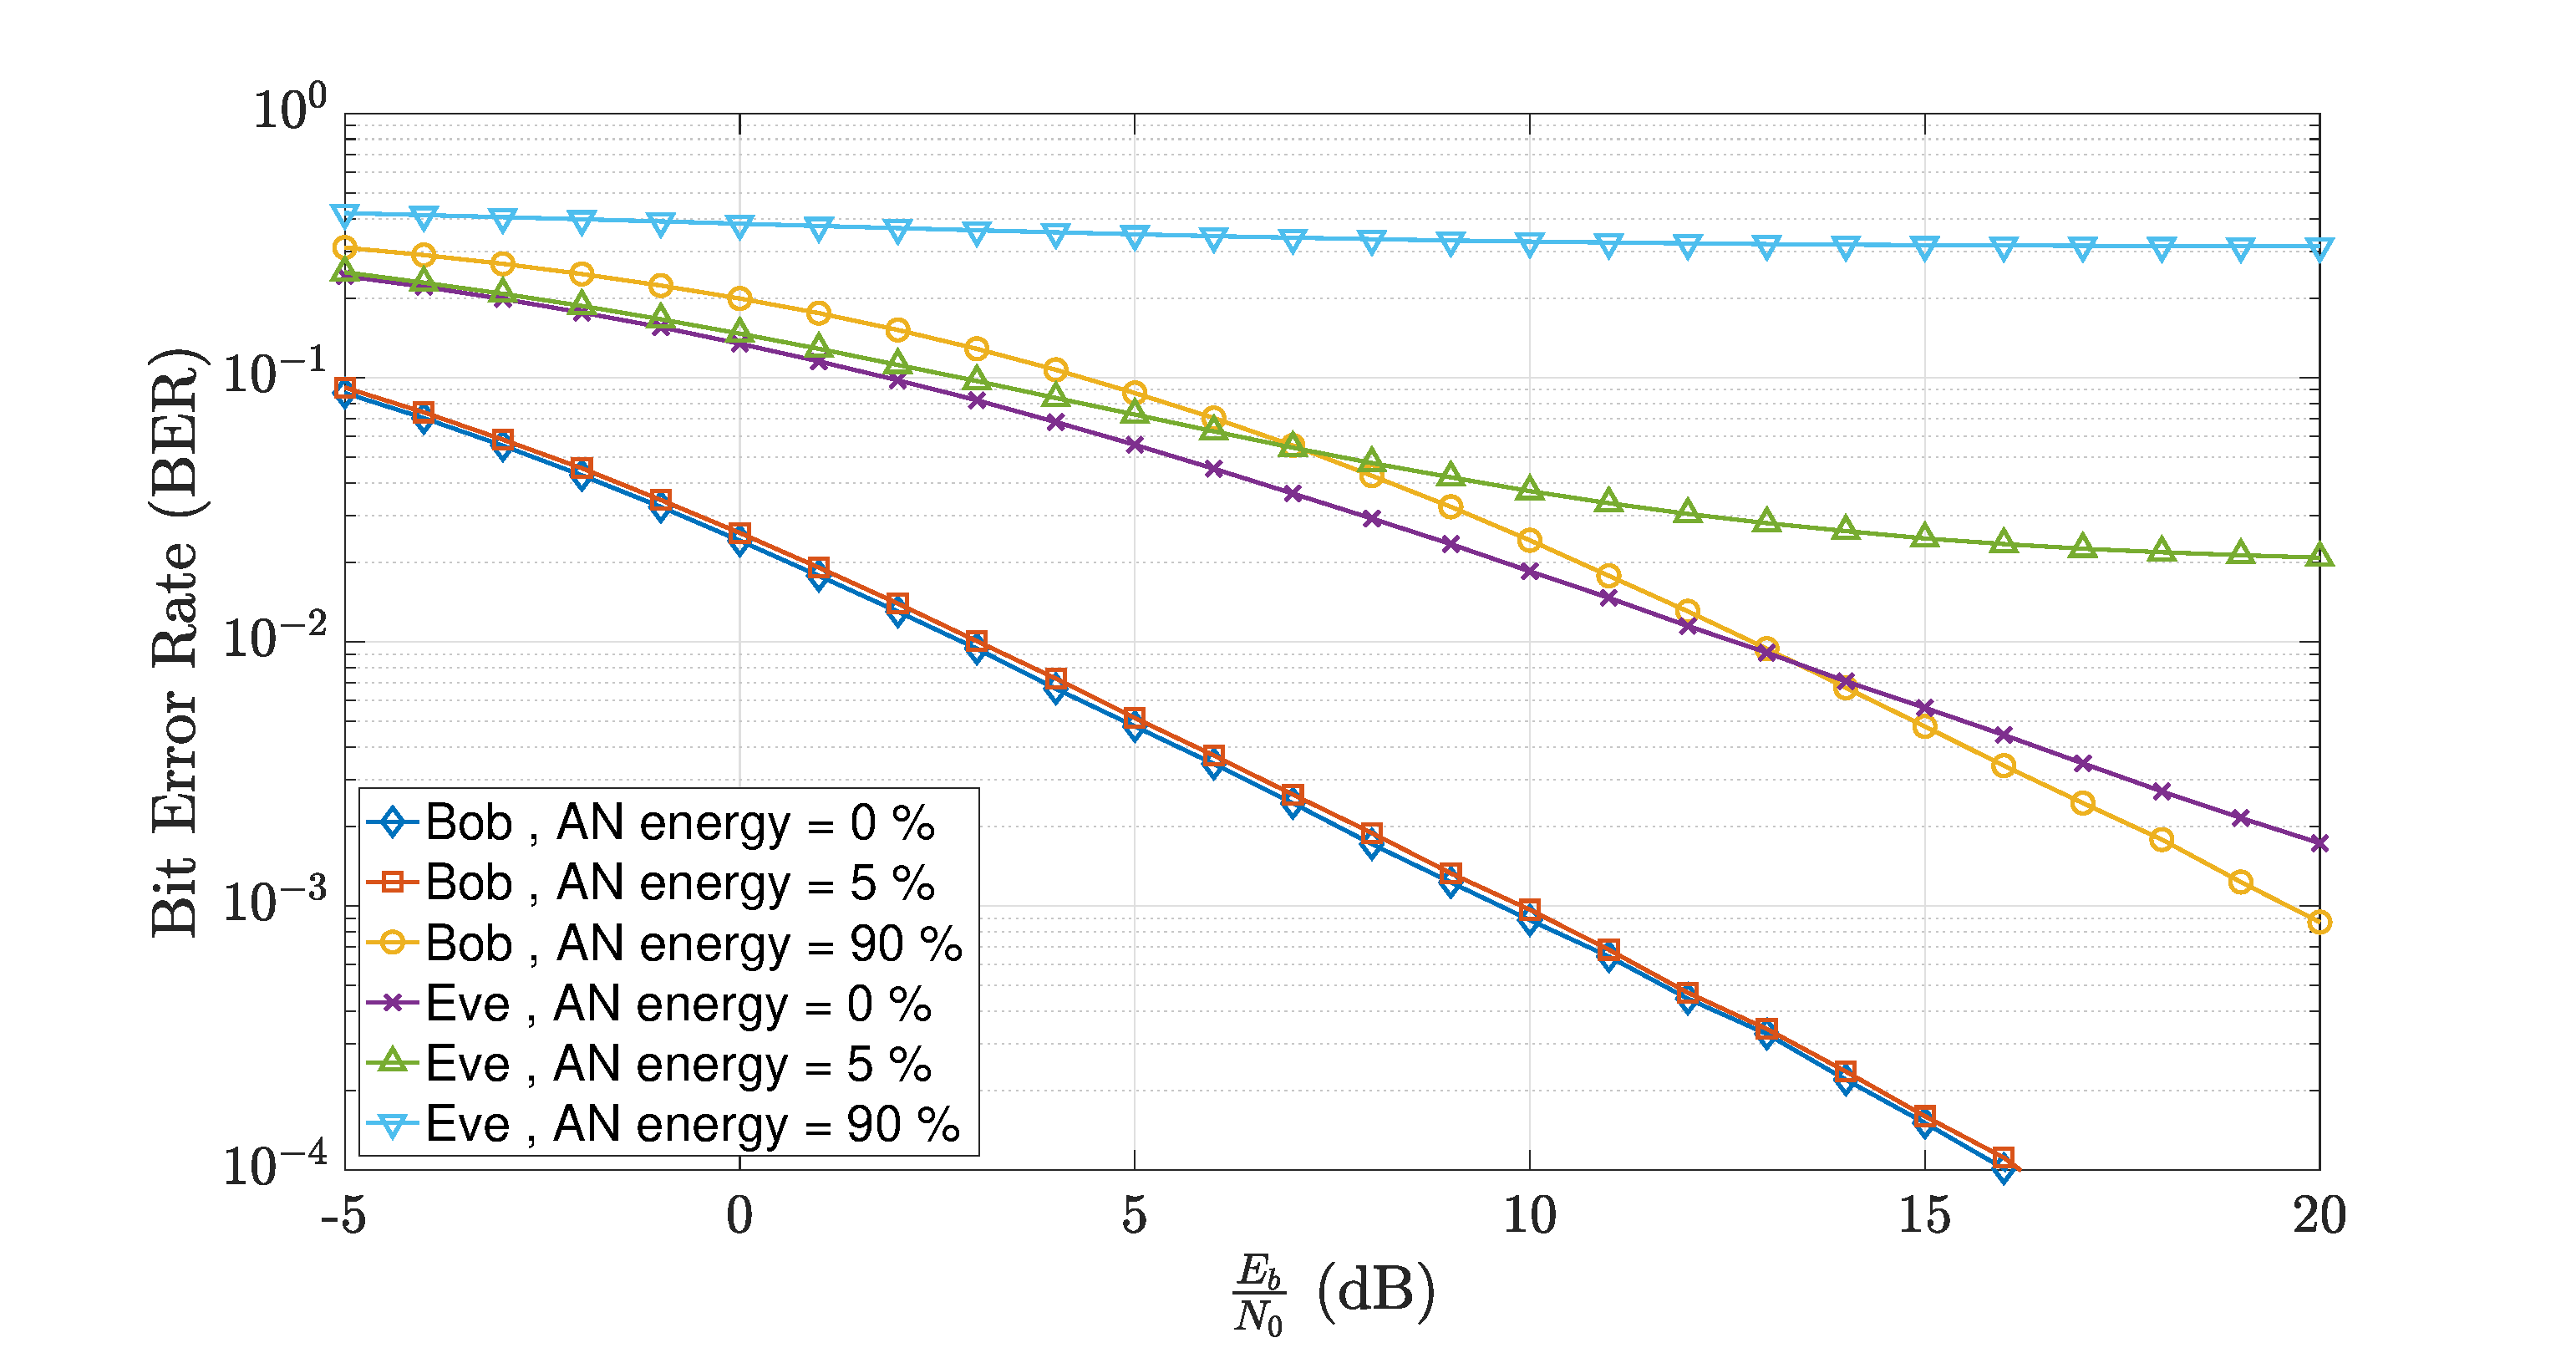
\includegraphics[width = .65\textwidth]{graphs/ber_ebno_alpha_bor_globcom.eps}}
    \caption{BER as a function of the level of noise for different AN energy values, \gls{bor} = 4}
    \label{fig:ber_ebno}
\end{figure}

\begin{figure}[htb!]
    \centering
    \centerline{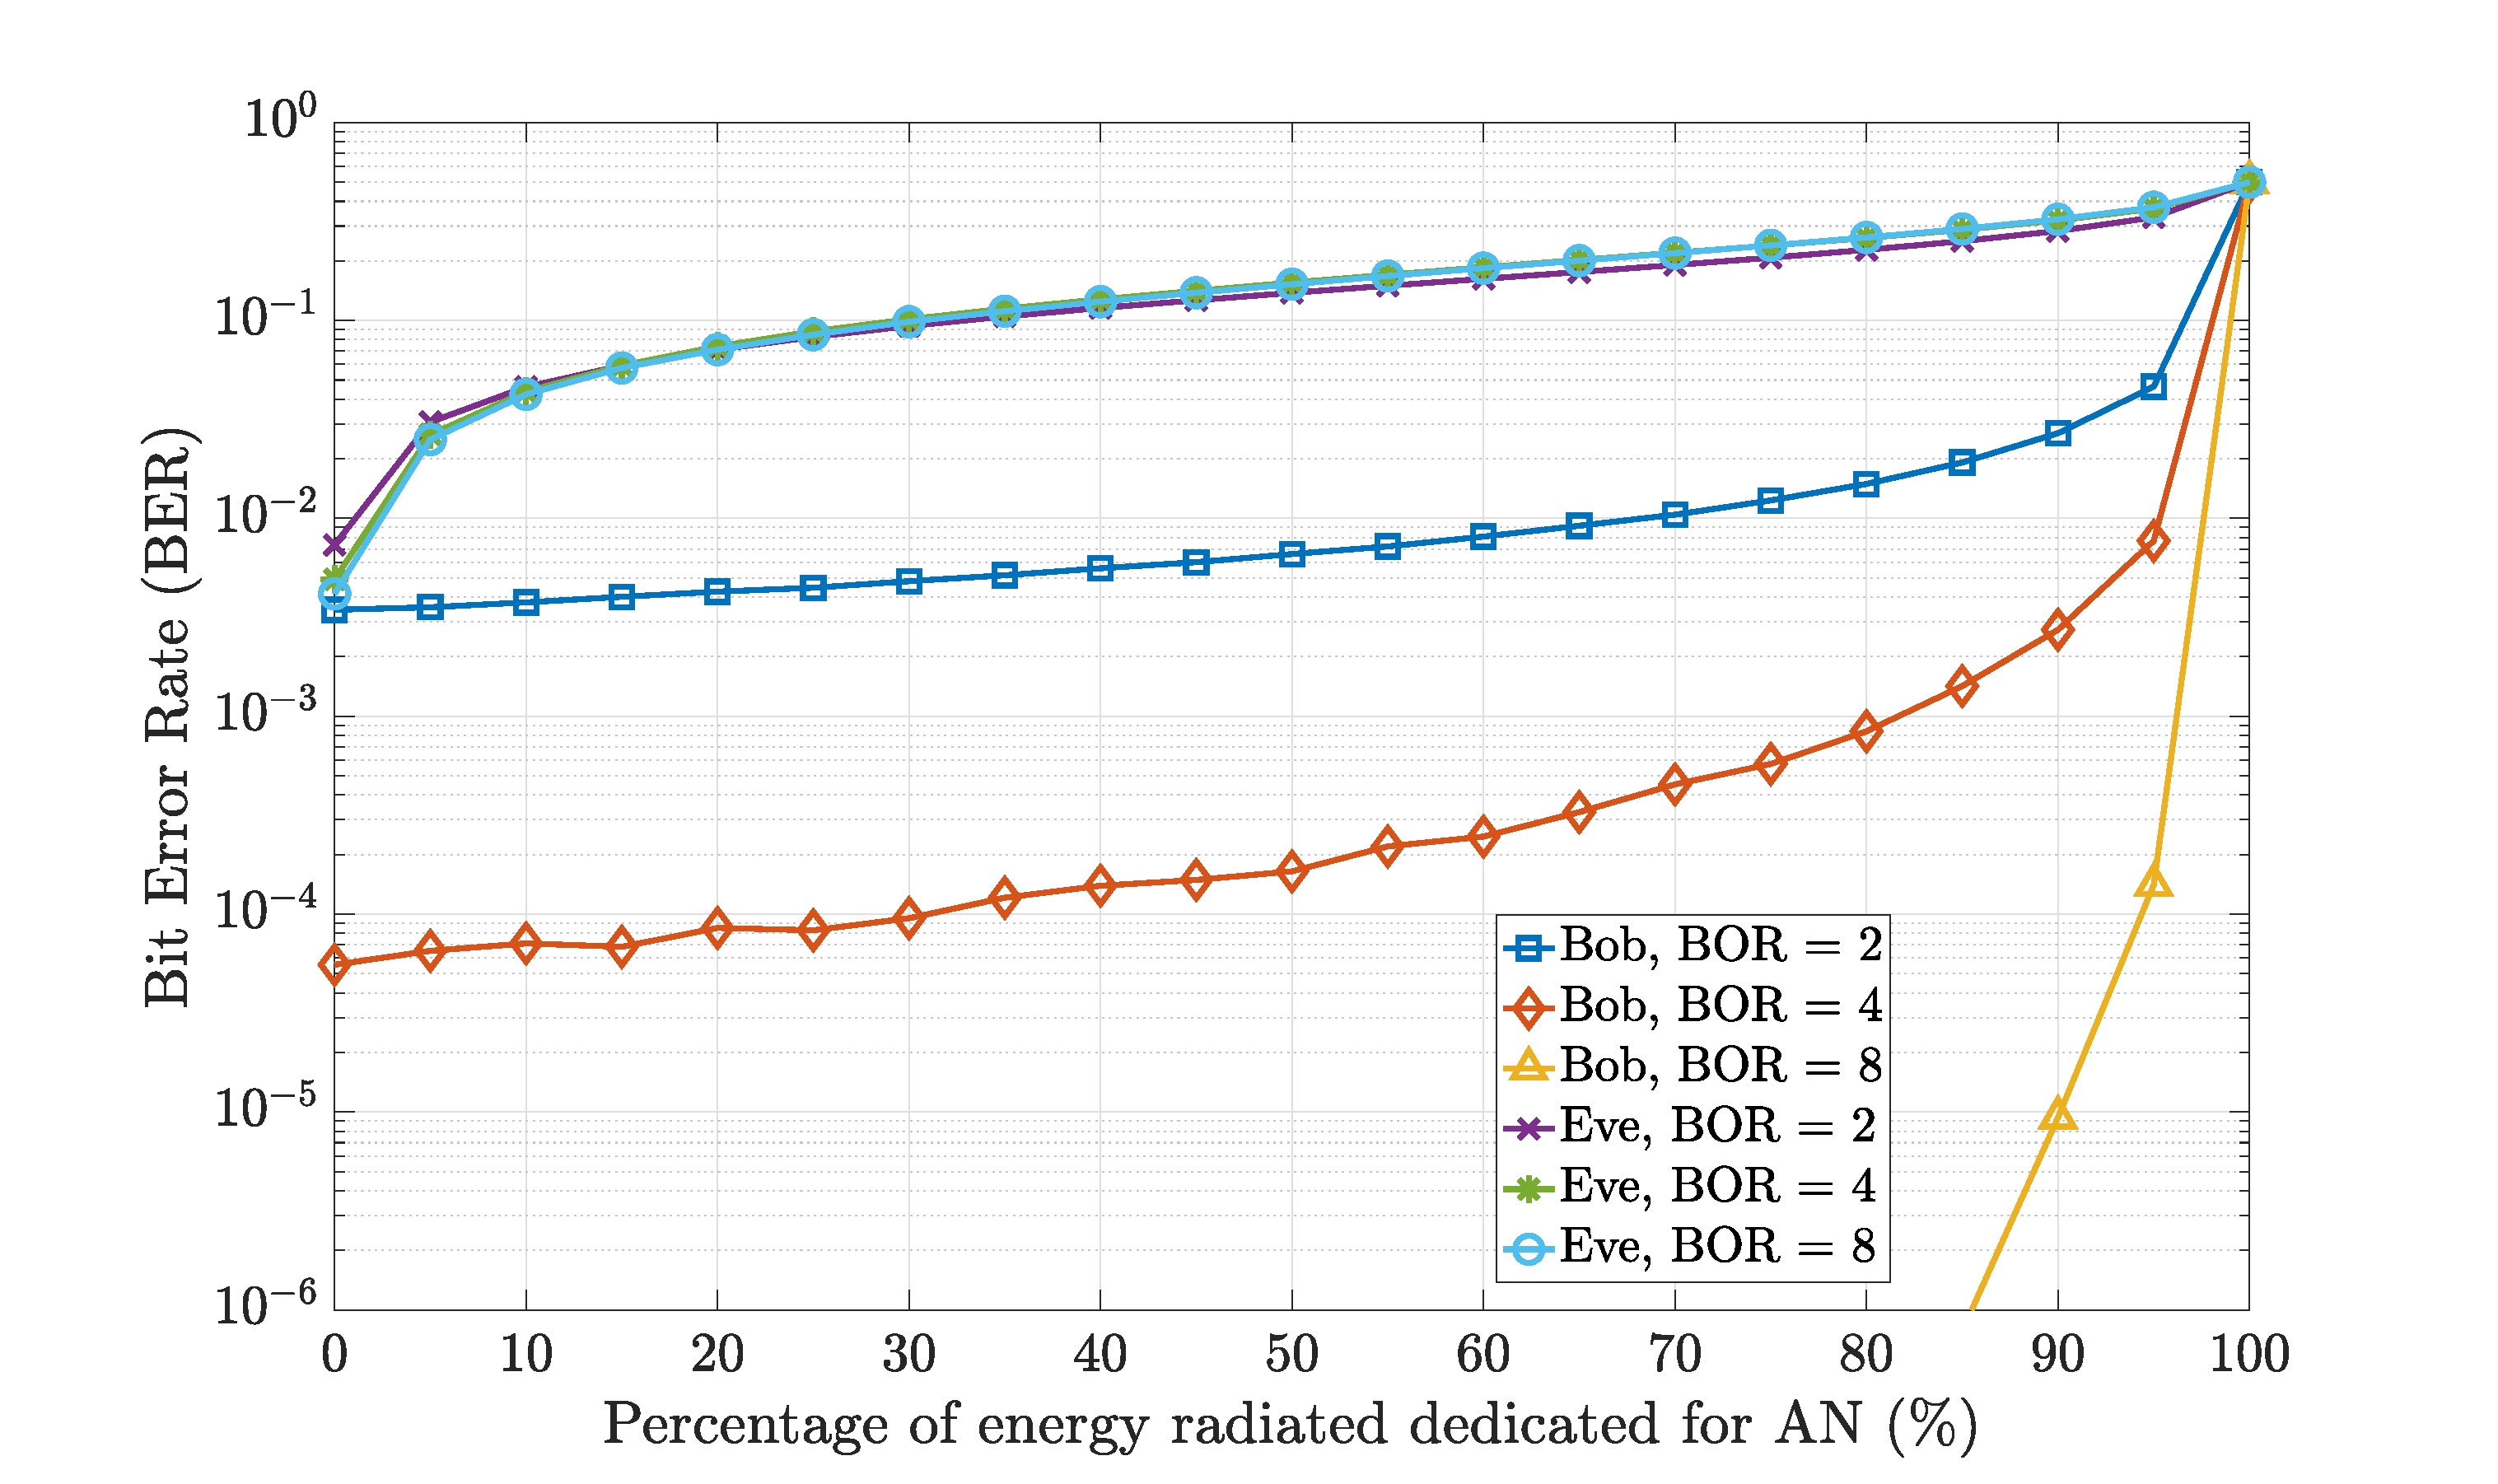
\includegraphics[width = .65\textwidth]{graphs/ber_alpha_bor_ebno_globcom.eps}}
    \caption{BER as a function of AN energy for different BOR values, $E_b/N_0 = 15$dB}
    \label{fig:ber_alpha}
\end{figure}
Fig. \ref{fig:ber_ebno} and \ref{fig:ber_alpha} show the system performance in terms of \gls{ber} obtained after \gls{zf} equalization at Bob and Eve. In Fig. \ref{fig:ber_ebno}, the \gls{ber} is plotted as a function of $E_b/N_0$, where $E_b$ is the energy per bit, calculated after spreading, and $N_0$ is the noise power spectral density.  Different levels of \gls{an} energy are investigated at fixed \gls{bor}. It can be observed that, as soon as a small amount of radiated energy is dedicated to \gls{an}, e.g., $5\%$, Eve's \gls{ber} strongly increases. At the intended position, the \gls{ber} also increases but much slower. The reason is that the higher the percentage of energy dedicated to \gls{an}, the lower the received useful signal power at Bob. In Fig. \ref{fig:ber_alpha}, the \gls{ber} is plotted as a function of the \gls{an} energy, at fixed $E_b/N_0=15$ dB and different \gls{bor} values. At the unintended position, the \gls{ber} naturally increases with the amount of injected \gls{an}, whatever the \gls{bor} value. At Bob, low \gls{ber} values can be maintained for high \gls{an} power by increasing the \gls{bor}. One can notice that, when $\alpha \to 0$, the \gls{ber} curves all converge to $0.5$, as expected.






\subsection{Secrecy results}
\label{subsec:sec_result}
\subsubsection{Eve and Bob with identical capacities}
\label{subsubsec:sec_result_despreading}
\begin{figure}[ht!]
    \centering
    \centerline{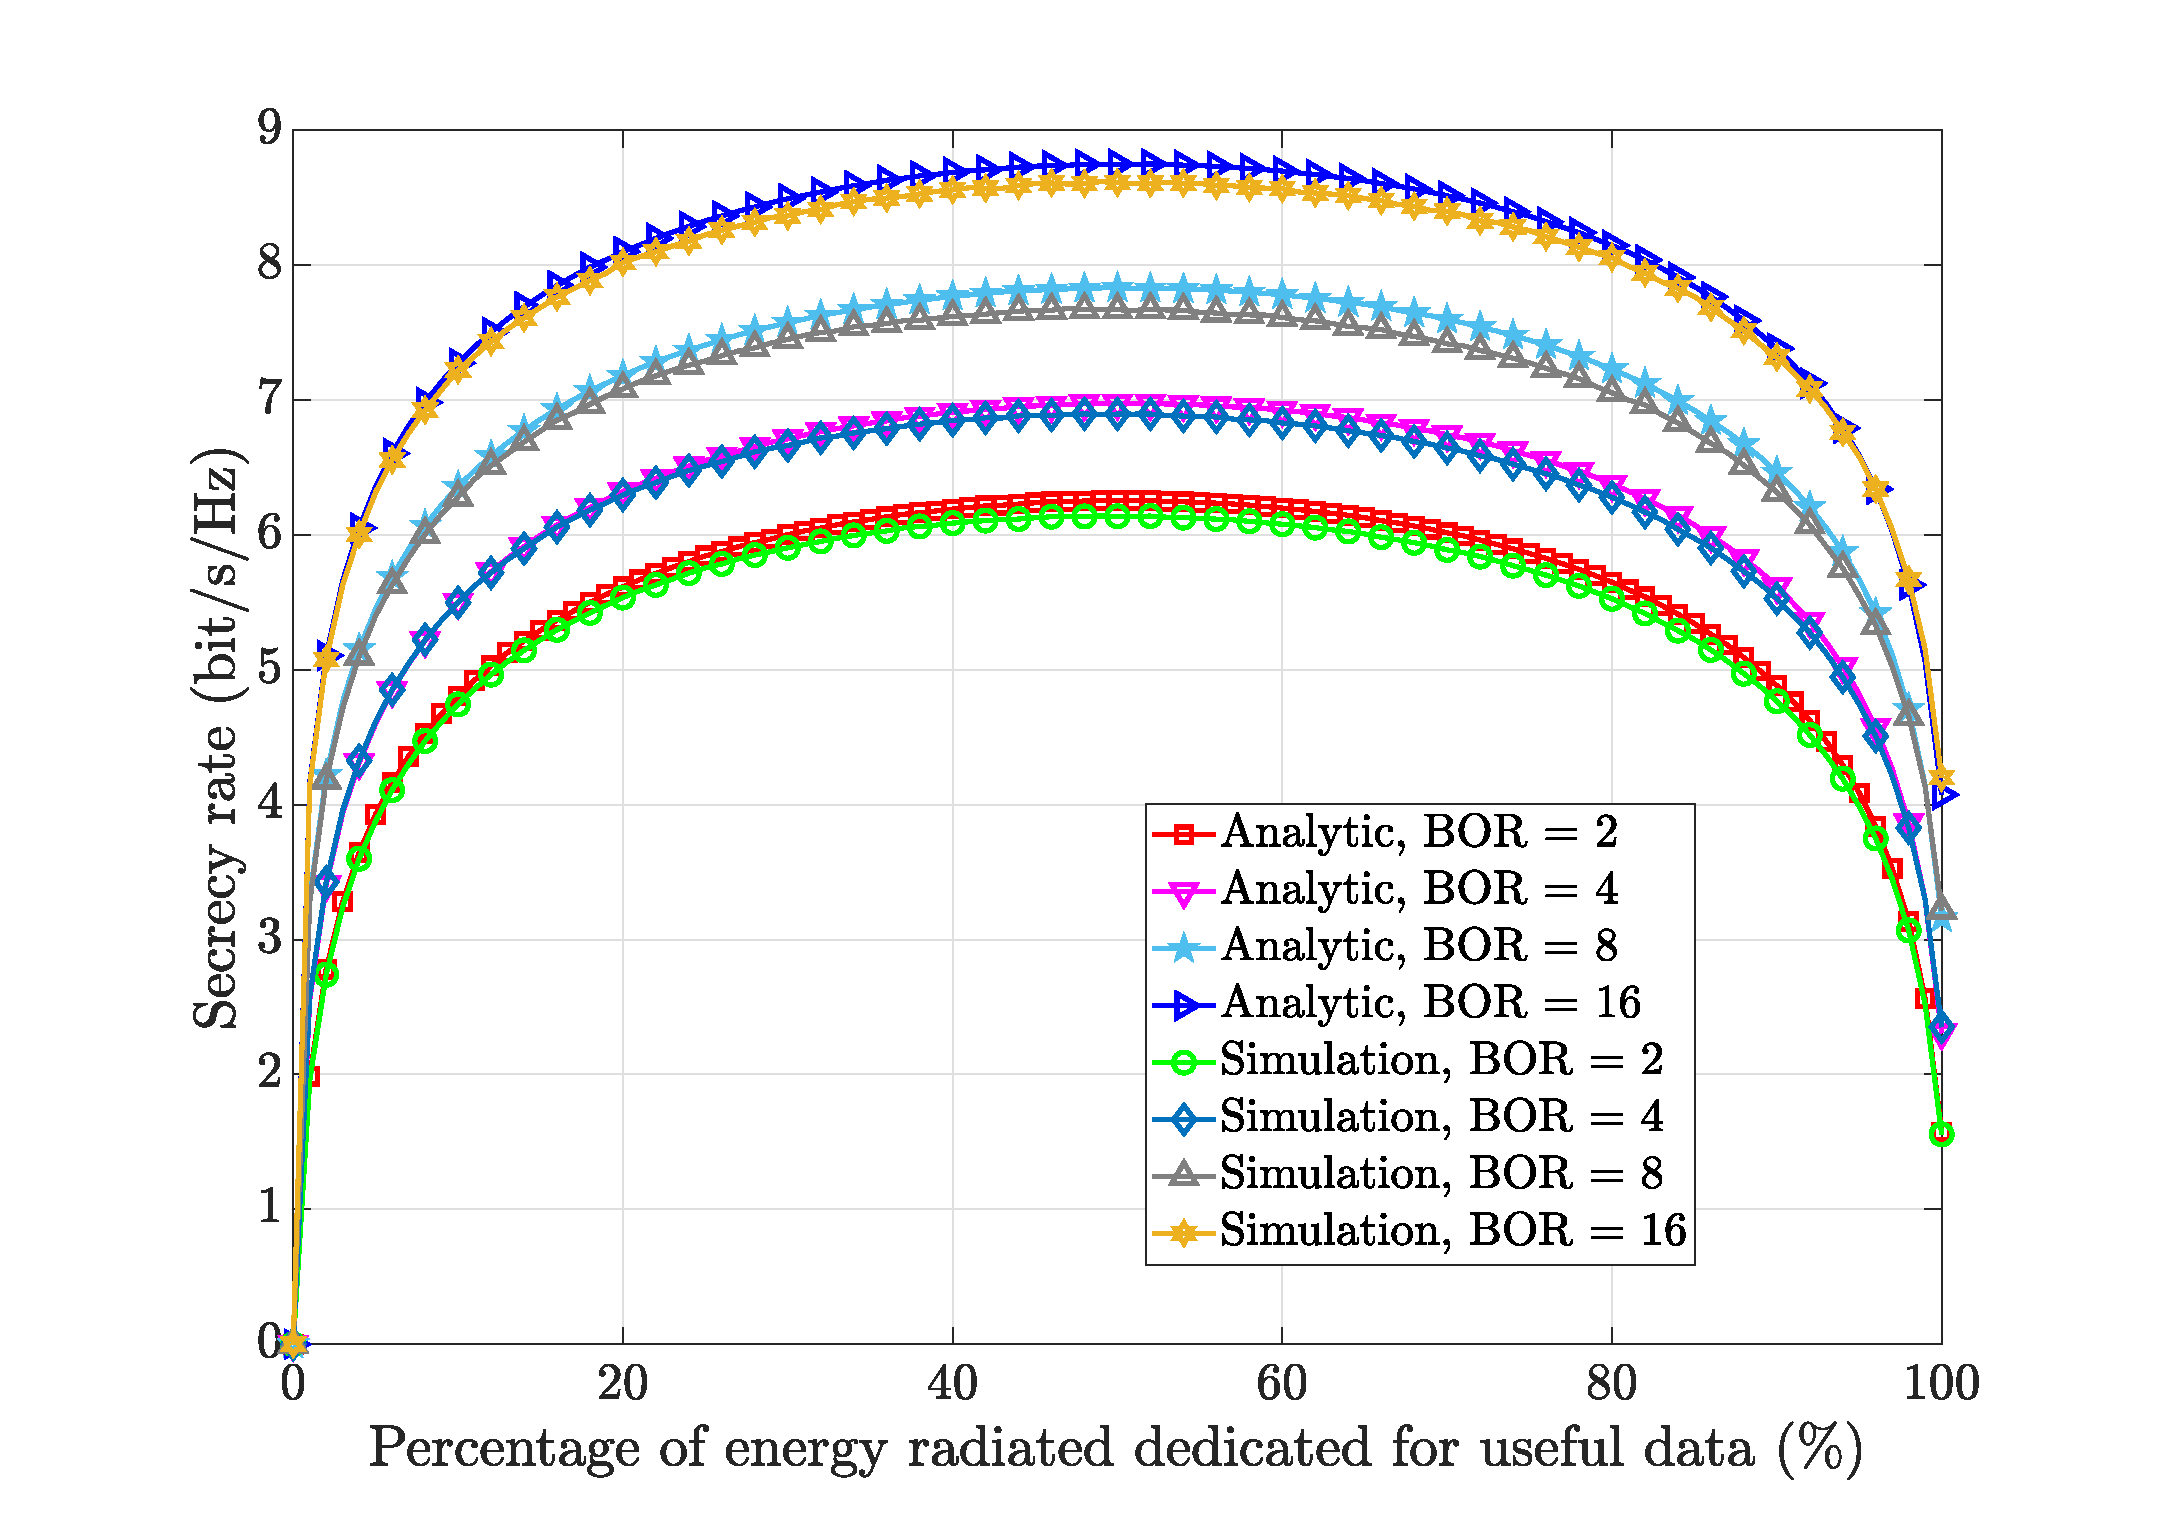
\includegraphics[width = .65\textwidth]{graphs/SR_simu_anal_filt0.eps}}
    \caption{Secrecy Rate curves, analytic vs simulation, Bob and Eve with same capabilities, $E_b/N_0=20$ dB }
    \label{fig:secrecy_alpha_bor}
\end{figure}
\begin{figure}[ht!]
    \centering
    \centerline{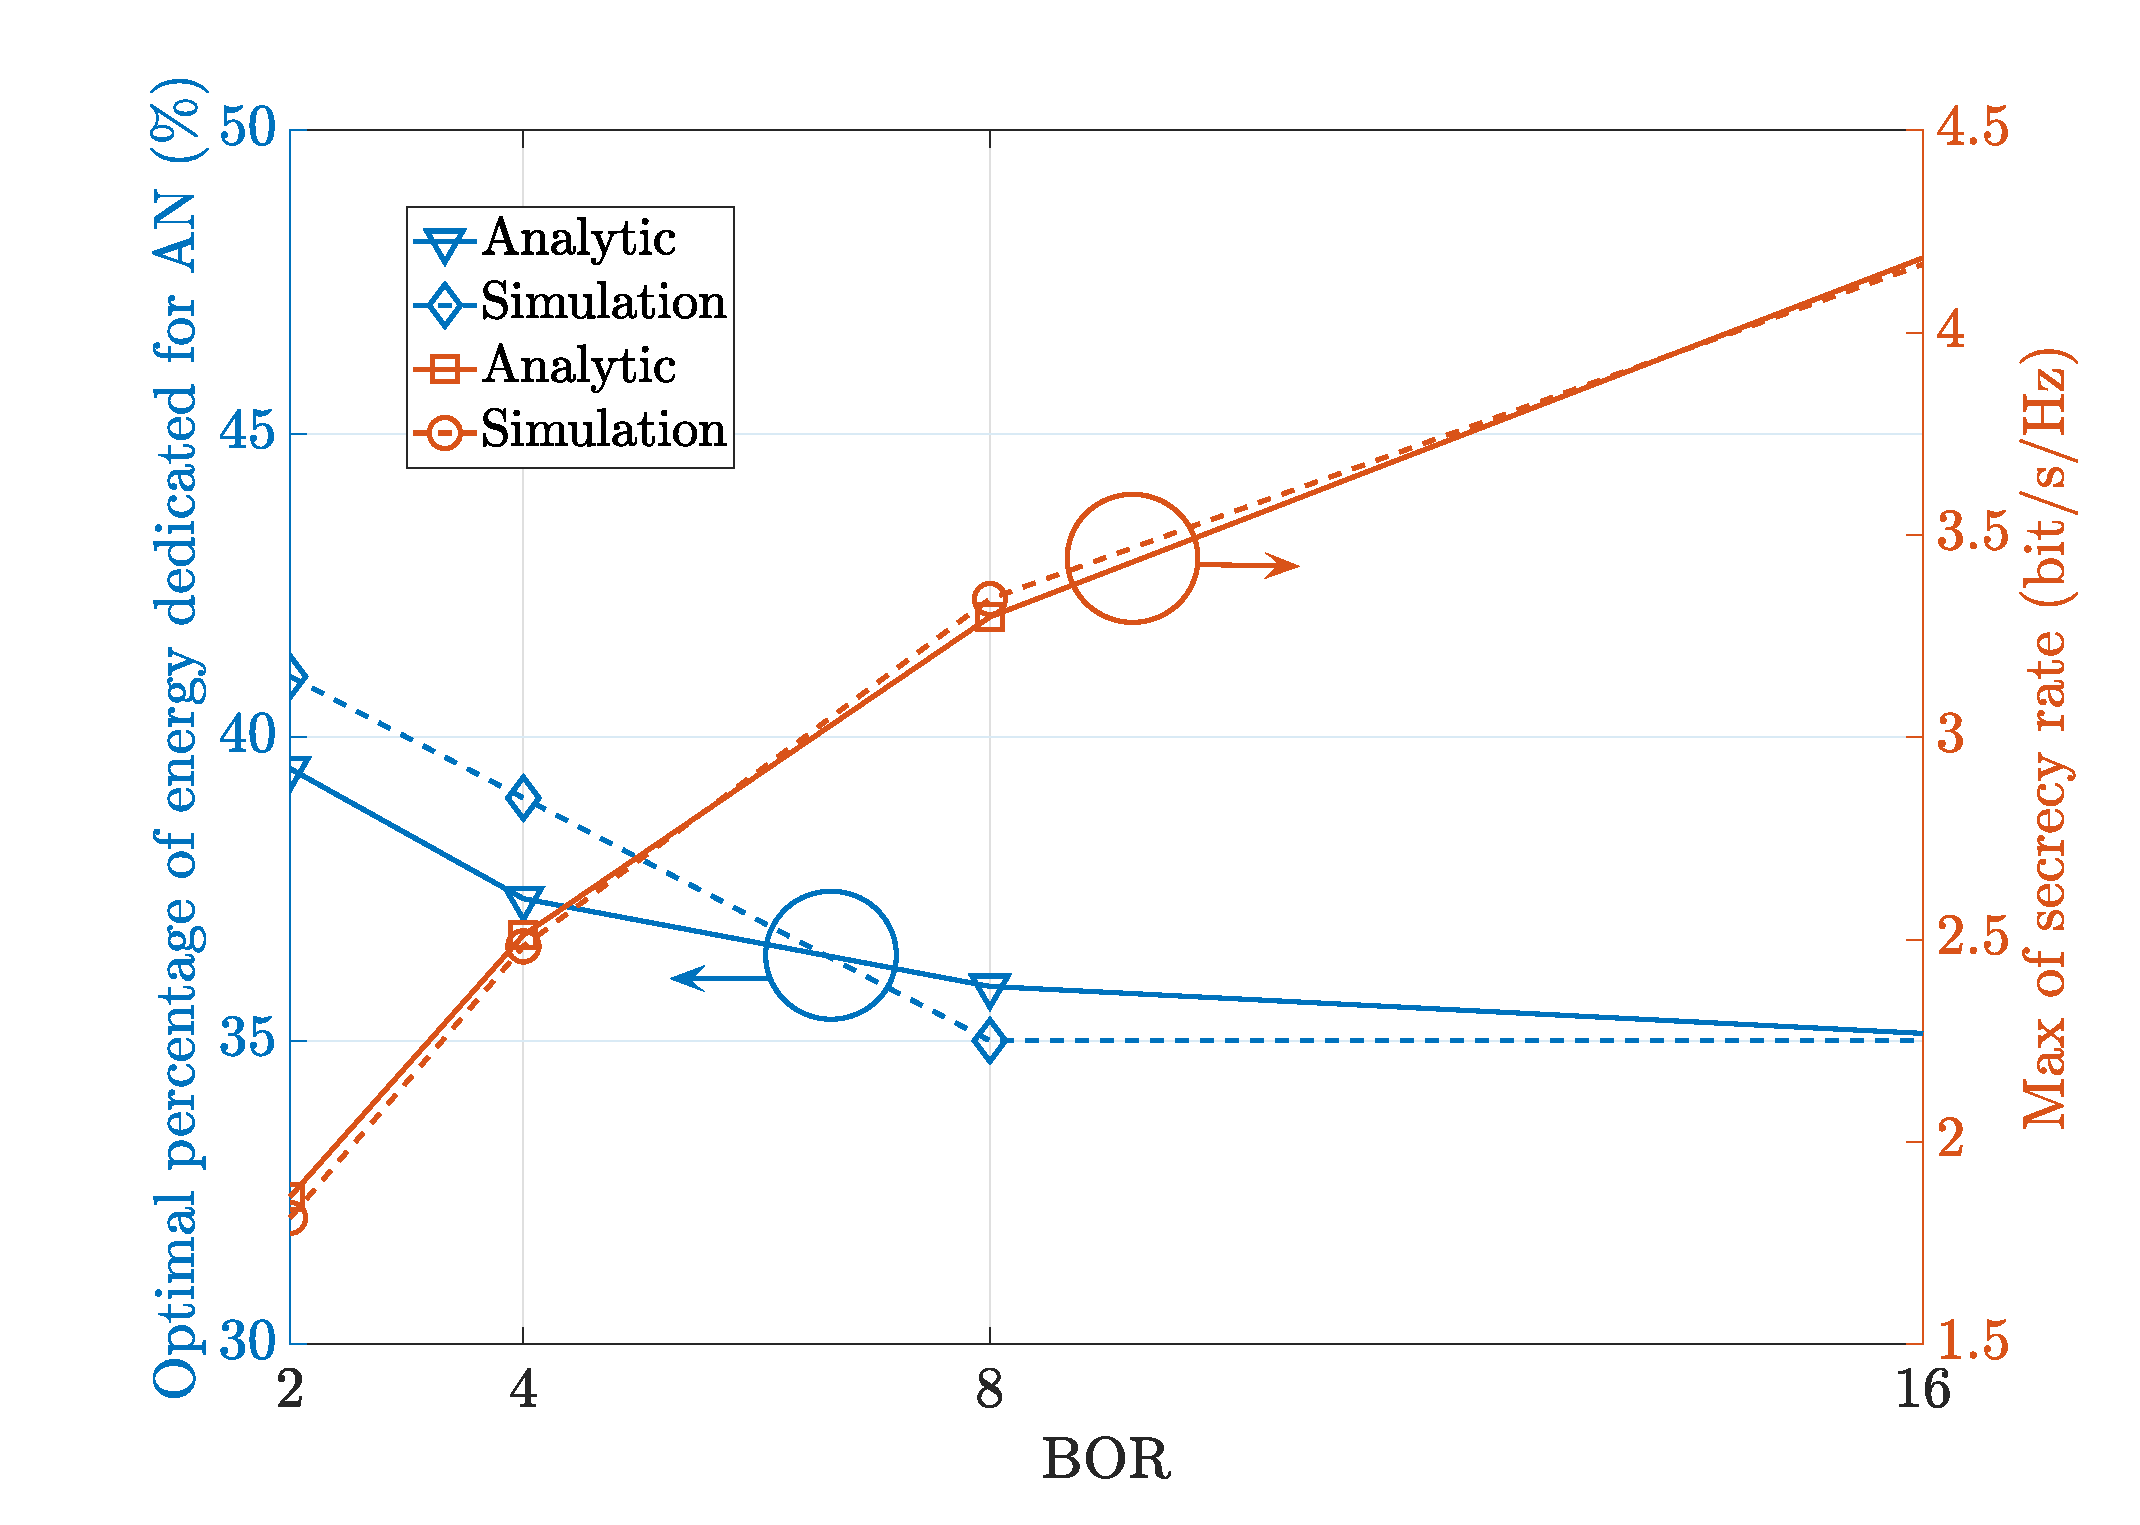
\includegraphics[width = .65\textwidth]{graphs/SR_max.eps}}
    \caption{Optimal amount of AN to inject, Bob and Eve with same capabilities, $E_b/N_0=5$ dB }
    \label{fig:secrecy_alpha_bor_optimal}
\end{figure}
Fig. \ref{fig:secrecy_alpha_bor} shows the \gls{sr} evolution as a function of $\alpha$ for different \gls{bor} values. It is considered that Eve's receiver is equivalent to Bob's one. First, it can be seen that analytic curves, given by (\ref{eq:SR_anal2}), approximate well the simulation curves and remains a tight upper bound for all scenarios.  In addition, the \gls{sr} obtained with the classical \gls{fd} \gls{tr} \gls{siso} \gls{ofdm} system, i.e., no \gls{an} signal, is enhanced with the addition of \gls{an} except for very high percentages of \gls{an}. Furthermore, the \gls{sr} increases when the \gls{bor} becomes higher because the \gls{tr} gain becomes larger at Bob for higher \gls{bor} values but not at Eve. No more secrecy is obtained when $\alpha \to 0$, since the \gls{sinr}'s at Bob and Eve drop to zero.\\
Fig. \ref{fig:secrecy_alpha_bor_optimal} illustrates the values of $\alpha_{opt}$ given by (\ref{eq:best_alpha}) that maximize the \gls{sr} determined from the closed-form approximation (\ref{eq:SR_anal2}), as well as obtained from the numerical simulations. The analytic estimation of the optimal amount of \gls{an} energy is not perfect but, the resulting simulated \gls{sr} is very close to the maximal \gls{sr}. The reason can be observed in Fig. \ref{fig:secrecy_alpha_bor} where the \gls{sr} varies very slowly about its maximum when $\alpha$ changes. So, for a given \gls{bor} value, Alice can make a rough determination of $\alpha_{opt}$ and therefore the available \gls{sr}, if $E_b/N_0$ is known.  







\subsubsection{Comparison between the different decoding structures}
\begin{figure}[htb!]
    \centering
    \centerline{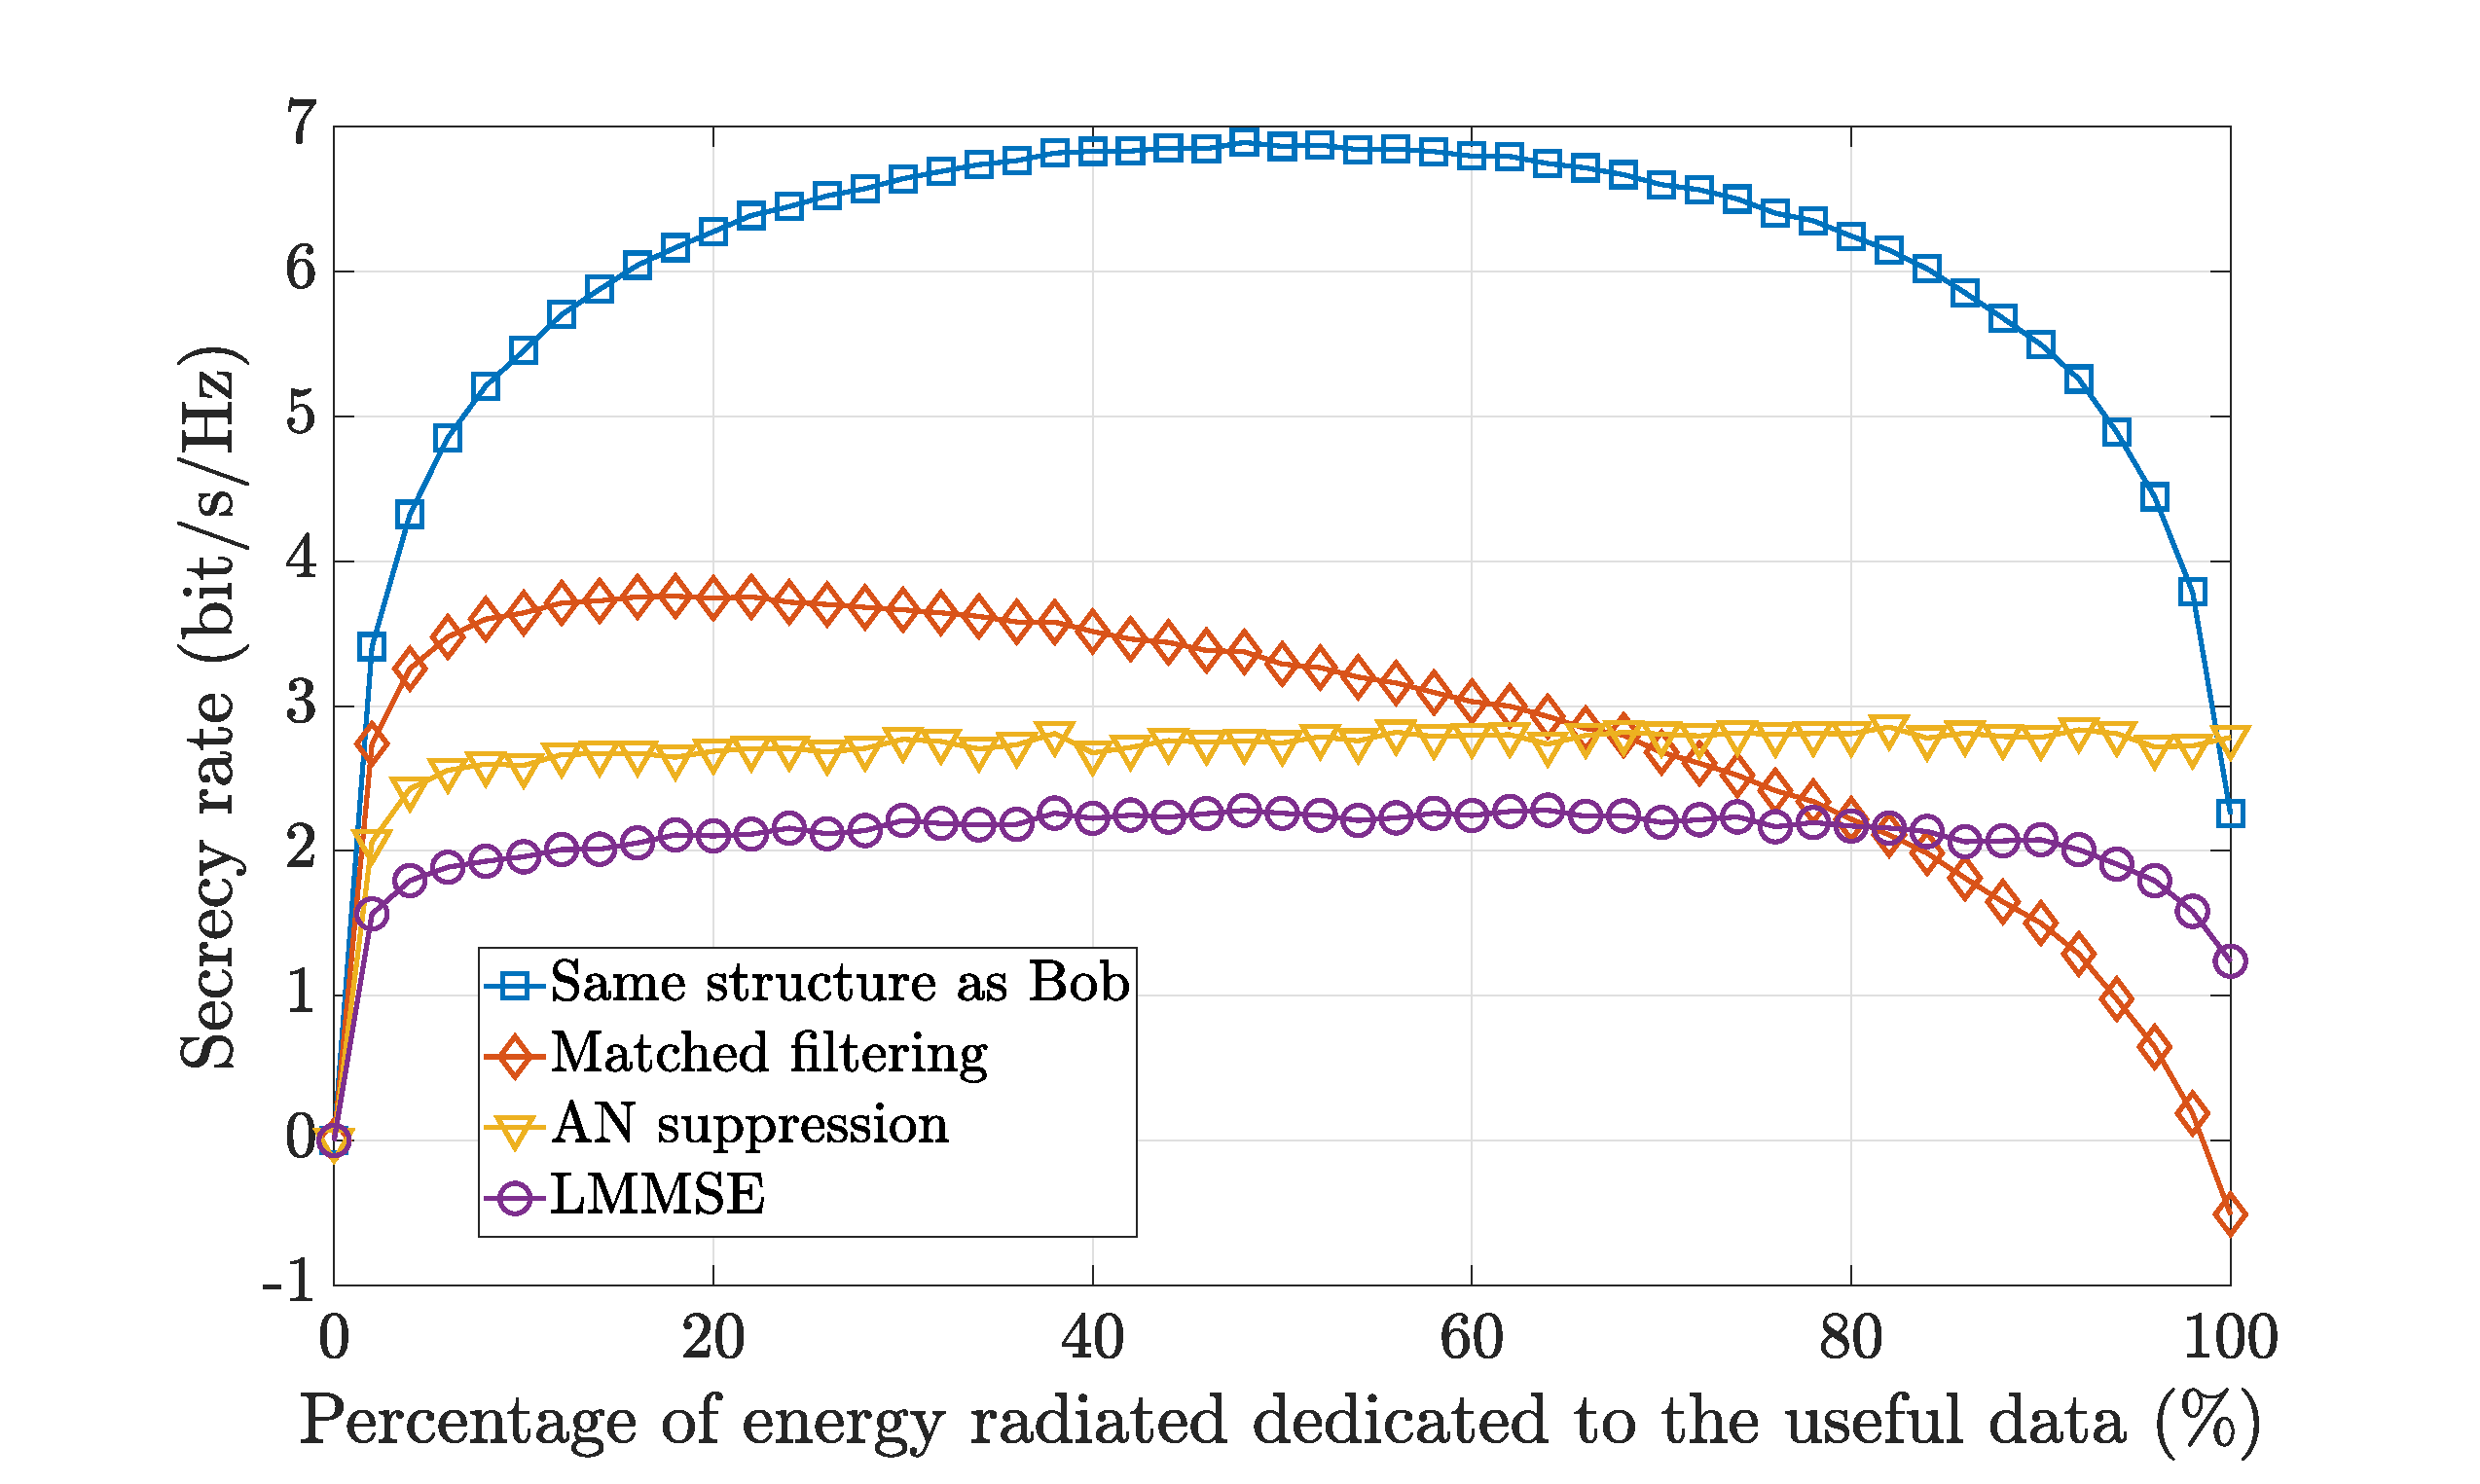
\includegraphics[width = .65\textwidth]{graphs/SR_filter_comparaison.eps}}
    \caption{Secrecy Rate curves for the different decoding structures at Eve, $E_b/N_0=20$ dB, BOR = 4 }
    \label{fig:secrecy_filt_comparaison}
\end{figure}
Fig.\ref{fig:secrecy_filt_comparaison} shows the secrecy performances for the 4 different structures implemented at the eavesdropper position, each of them assuming more computational resources and/or more knowledges at Eve as compared to Bob. It can be seen that when Eve implements the same receiving structure as Bob, the \gls{sr} is very high compared to the other curves, as anticipated from Section \ref{par:eve_same_bob}. When the \gls{an} killer algorithm is implemented, we observe that the curve remains flat, except for the situation where all the radiated energy is dedicated for the \gls{an} signal. The reason is that Eve's noise is amplify whatever the value of $\alpha$ since the \gls{an} signal is suppressed. The \gls{lmmse} curves exhibit the lower \gls{sr} sice it performs a decoding tradeoff between suppressing the \gls{an} and amplifying its noise, except for very high percentages of energy dedicated to the useful signal. Finally, we note that the \gls{sr} when Eve implements a matched filter is relatively low. Furthermore, it becomes negative when the transmitted signal only contains data. In fact, if Eve and Bob noise levels are identical, which is assumed throughout this report , the \gls{sinr} ratio when no \gls{an} is radiated becomes:
\begin{equation}
    \kappa \approx \frac{\EX{\gamma_{B,n}}}{\EX{\gamma_{E,n}}}\Big|_{\alpha \to 1} \approx \frac{\frac{U+1}{U}}{\left(\frac{U+1}{U}\right)^2} = \frac{U}{U+1}< 1
\end{equation}
giving rise to a negative \gls{sr}. The reason why the \gls{lmmse} decoding structure does not exhibit better decoding performances at Eve, i.e., lower \gls{sr} values, compared to the matched filter receiver for all values of $\alpha$ has not been explained yet.






\subsubsection{Waterfilling Optimization}
\label{subsub:simu_waterfilling}
\begin{figure}[htb!]
    \centering
    \centerline{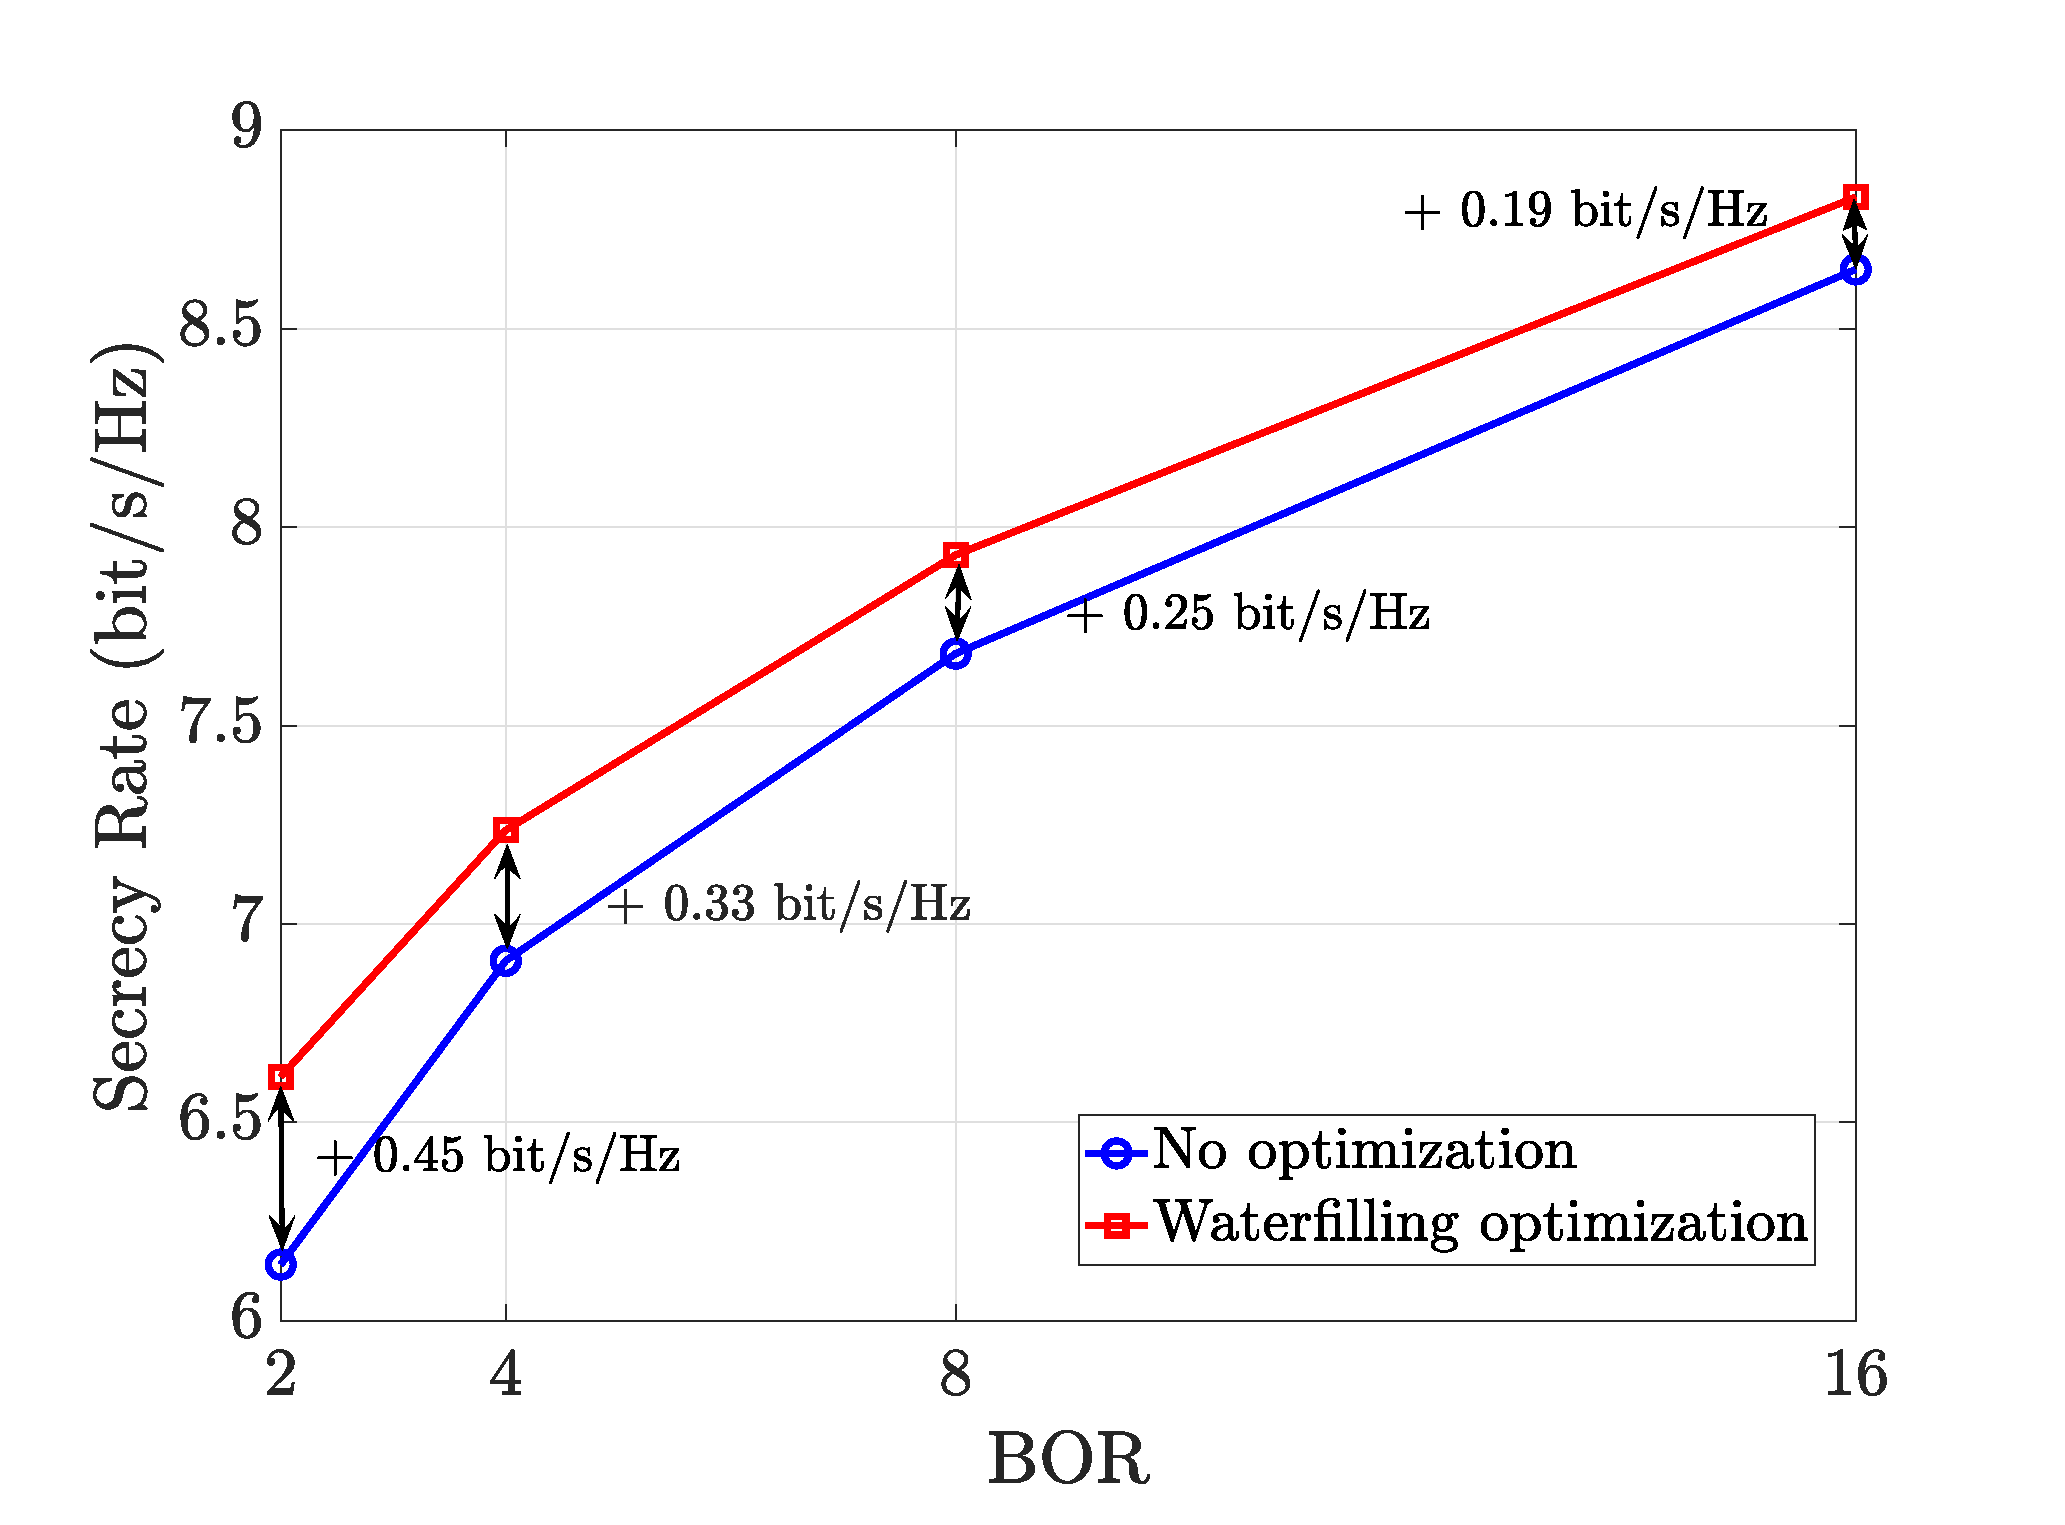
\includegraphics[width = .65\textwidth]{graphs/alpha_waterfilling.eps}}
    \caption{SR optimization via waterfilling, Bob and Eve with same capabilities, $E_b/N_0=20$ dB}
    \label{fig:waterfilling_opt_alpha}
\end{figure} 
Fig. \ref{fig:waterfilling_opt_alpha} presents the maximal values of the \gls{sr} obtained when Eve implements the despreading only receiving structure, i.e. the same structure as Bob, before and after waterfilling optimization. As a reminder, before and after optimization, the mean energy radiated dedicated to the useful data remains unchanged. This amount of energy is computed thanks to (\ref{eq:best_alpha}) in order to ensure a maximal \gls{sr}. This \gls{sr} is then further increased via the waterfilling optimization procedure, as described in section \ref{subsec:perf_waterf}. As we can see, there is an increase of the \gls{sr} for all \gls{bor} values thanks to the optimization. However, this increase decreases with an increase of the \gls{bor}. This can be explained since, when the \gls{bor} increases, the channel frequency diversity is better exploited by the \gls{tr} scheme. Therefore, it becomes more difficult to gain from the coefficient optimization procedure and the \gls{sr} is then less enhanced. 
\section{Conclusion \& Perspectives}
\label{sec:ccl}
The problem of securing the \gls{fd} \gls{tr} \gls{siso} \gls{ofdm} wireless transmission from a transmitter to a legitimate receiver in the presence of a passive eavesdropper is considered. A novel and original approach based on the addition of an \gls{an} signal onto \gls{ofdm} blocks that improves the \gls{pls} is proposed. This approach can be easily integrated into existing standards based on \gls{ofdm}. It only requires a single transmit antenna and is therefore well suited for devices with limited capabilities. Analytic and simulation results show that the novel approach significantly improves the security of the communication and so considerably jeopardizes any attempt of an eavesdropper to retrieve the data. \\

In this work, four eavesdropper decoding structures are investigated giving rise to different secrecy performances. From the previous discussion, we remark that a simple matched filtering decoding structure strongly impacts the secrecy rate of the communication. As a result, one of the aspects of the future work will be to implement a more robust scheme. New \gls{an} injection methods and/or new precoding techniques will be investigated to try to further improve the security of the communication. \\

So far, only a \gls{siso} system has been considered. A natural extension of the work will be to consider a \gls{mimo} system. That way, in addition to benefiting from the  frequency diversity of the channels, we will benefit from the spatial diversity. In doing so, any attempt to try to eavesdrop the data will be expected to become harder. In addition, we will consider that the passive eavesdropper will be equipped with multiple antennas which will gives him more decoding capabilities. \\

Furthermore, only a single-user communication is now considered. A multi-users scheme can be designed where each user channel can contribute to secure the whole communication. As a consequence, the level of security of the scheme is expected to improve.\\

At this point of the work, a very simple channel model was implemented. In fact, a multi-taps channel where each tap is Rayleigh distributed is considered. No correlation between the different subcarriers, i.e. frequency correlation, or spatial correlation between Bob and Eve channels have been taken into account. This leads to results that are relatively easy to compare with analytic models but that do not represent well real life scenarios. A natural extension of the work will be to consider these correlations in order to obtain more realistic results. \\

Finally, the objective will be to test the \gls{fd} \gls{tr} \gls{ofdm} system with the \gls{usrp} devices in real indoor environments.
\label{sec:ccl}



% %%%%%%%%%%%%%%%%
% BIBLIOGRAPHY %
%%%%%%%%%%%%%%%%

\newpage
\bibliographystyle{IEEEtran}
\bibliography{biblio} 
%% ----------------------------------------------------------------
% Now begin the Appendices, including them as separate files
%% ----------------------------------------------------------------

\backmatter

\appendix % Cue to tell LaTeX that the following 'chapters' are Appendices
\makeatletter
\renewcommand{\thesection}{\theparagraph\@arabic\c@section}
\makeatother
\section*{Appendices}
\renewcommand\thefigure{\thesection\arabic{figure}}    
\counterwithin{figure}{section}
\counterwithin{table}{section}
%\renewcommand{\thesection}{\Alph{section}.\arabic{section}}

\begin{appendices}
%\renewcommand{\appendixtocname}{Annexes} 
\addcontentsline{toc}{section}{Appendices}



% ANNEXE A : SINR determination
\setcounter{figure}{0}
\setcounter{table}{0}
\setcounter{section}{0}
\setcounter{equation}{0}
\numberwithin{equation}{section}
\renewcommand{\theparagraph}{A}

\section{SINR derivation}\label{appA:SINR_deriv}
Let $A$ and $B$ be 2 \gls{rv}'s. These basics properties will be used:
\begin{equation}
    \begin{split}
        &\EX{\alpha A + \beta B} = \alpha \EX{A} + \beta \EX{B} \; \;\; \;\alpha,\beta\in\R \\
        &\EX{AB} = \EX{A} \EX{B} \; \;\; \; \text{if $A$ and $B$ are independent} \\
        &\EX{AB} = \EX{A} \EX{B} + \text{cov}(A,B)\; \; \; \;\text{if $A$ and $B$ are correlated}
    \end{split} 
\end{equation}
\subsection{At the intended position}
As a recall, the received sequence is given by:
\begin{equation}
    \textbf{y}_{\text{B}}^H = \sqrt{\alpha} \; \spread^H \module{\HB}^2 \spread \textbf{x} \;  +  \;  \spread^H \textbf{v}_\text{B} 
    \label{eq:app:rx_bob_AN}
\end{equation}

\paragraph*{Data component}
From (\ref{eq:RV_sinr_b}) and (\ref{eq:expected_bob}), we have:

\begin{subequations}
    \begin{align}
        \EX{|k|^2} &= \EX{\module{\sqrt{\alpha}\spread^H \module{\HB}^2 \spread}^2} \\
        \EX{|k_n|^2} &=\EX{\left|\frac{\sqrt{\alpha}}{U}\sum_{i=0}^{U-1} \left| h_{\text{B}, n + iN}\right|^2\right|^2}  \\
        &= \frac{\alpha}{U^2} \EX{\left(\sum_{i=0}^{U-1} \left| h_{\text{B}, n + iN}\right|^2\right) \left(\sum_{j=0}^{U-1} \left| h_{\text{B}, n + jN}\right|^2\right)^H} \label{subeq:appA:comp1}\\
        &= \frac{\alpha}{U^2}\EX{\sum_{i=0}^{U-1}\sum_{j=0}^{U-1}\left| h_{\text{B}, n + iN}\right|^2 | h^*_{\text{B}, n + jN}|^2} \\
        &= \frac{\alpha}{U^2}\EX{\sum_{i=0}^{U-1}\left| h_{\text{B}, n + iN}\right|^4 + \sum_{i=0}^{U-1}\sum_{\substack{j=0 \\ j\neq i}}^{U-1}\left| h_{\text{B}, n + iN}\right|^2 | h^*_{\text{B}, n + jN}|^2} \\
        &= \frac{\alpha}{U^2} \left(\EX{\sum_{i=0}^{U-1}\left| h_{\text{B}, n + iN}\right|^4} + \EX{\sum_{i=0}^{U-1}\sum_{\substack{j=0 \\ j\neq i}}^{U-1}\left| h_{\text{B}, n + iN}\right|^2 | h^*_{\text{B}, n + jN}|^2} \right) \\
        &=  \frac{\alpha}{U^2} \left(\EX{\sum_{i=0}^{U-1}\left| h_{\text{B}, n + iN}\right|^4} + \EX{\sum_{i=0}^{U-1}\left| h_{\text{B}, n + iN}\right|^2}\EX{\sum_{\substack{j=0 \\ j\neq i}}^{U-1} | h^*_{\text{B}, n + jN}|^2} \right) \label{eq:an_2g}\\
        &= \frac{\alpha}{U^2} \left( 2U + U(U-1)\right) = \frac{\alpha (U+1)}{U} \label{eq:an_2h}
    \end{align}
    \label{eq:appA:data_bob}
\end{subequations}
Going from (\ref{eq:an_2g}) to (\ref{eq:an_2h}) can be deduced from Appendix \ref{appC}. It is then easy to show that $\EX{\left| h_{\text{B}, n + iN}\right|^4}=2$. 

\paragraph*{Additive white gaussian noise component}
We compute the mean energy per symbol of the received noise signal:
\begin{subequations}
    \begin{align}
        \EX{|\textbf{v}_{\text{B}}|^2} &=  \EX{\module{\spread^H \vb}^2} \\
        &= \EX{\left(\spread^H \vb \right)\left(\spread^H \vb \right)^H} \\
        &=\EX{\spread^H \vb \vb^* \spread } \\
        \EX{|v_{\text{B,n}}|^2} &= \frac{1}{U} \EX{\sum_{i=0}^{U-1} |v_{\text{B}, n + iN}|^2} = \sigma^2_{\text{V,B}}
    \end{align}
    \label{eq:appA:noise_bob}
\end{subequations}

       % &\EX{|x_n|^2} = 1\\
       % &\EX{|v_{B,n}|^2} = \sigma^2_{V,E}



\subsection{At the unintended position}
At the unintended position, the received signal is given by:
\begin{equation}
    \textbf{y}_{\text{E}}^G = \sqrt{\alpha} \textbf{G}\Gamma_{\text{E}} \textbf{x} + \sqrt{1-\alpha} \textbf{G} \HE \w + \ve
    \label{eq:appA_rx_eve}
\end{equation}
where $\Gamma_{\text{E}} = \HE \HB^*\spread$




\subsubsection{Eve and Bob with identical capacities}
In this scenario, we have:
\begin{equation}
    \textbf{y}_{\text{E}}^G = \sqrt{\alpha} \spread^H \Gamma_{\text{E}} \spread\; \textbf{x} \; +  \; \sqrt{1-\alpha} \; \spread^H \HE \w  \; +  \; \spread^H  \textbf{v}_\text{E} 
    \label{eq:app:rx_eve_filt0}
\end{equation}


\paragraph*{Data component}
From (\ref{eq:expected_eve_filt0}), we have:
\begin{subequations}
    \begin{align}
        \EX{|\textbf{A}_{1}|^2} &= \EX{\module{\sqrt{\alpha}\spread^H \HE\HB^* \spread}^2} \\
        &= \alpha \EX{\left( \spread^H \HE\HB^* \spread \right) \left( \spread^H \HE\HB^* \spread\right)^H} \\
        \EX{|A_{1,n}|^2}&=\alpha \EX{\frac{1}{U^2} \sum_{i=0}^{U-1} \left| h_{\text{E}, n + iN} \right|^2 \left| h^*_{\text{B}, n + iN}\right|^2 } \\
        &= \frac{\alpha}{U}
    \end{align}
    \label{eq:appA:data_eve_filt0}
\end{subequations}

\paragraph*{Additive white gaussian noise component}
For the noise component:
\begin{subequations}
    \begin{align}
        \EX{|\textbf{A}_{2}|^2} &=  \EX{\module{\spread^H \ve}^2} \\
        &= \EX{\left(\spread^H \ve \right)\left(\spread^H \ve \right)^H} \\
        &=\EX{\spread^H \ve \ve^* \spread } \\
        \EX{|A_{2,n}|^2} &= \frac{1}{U} \EX{\sum_{i=0}^{U-1} |v_{\text{E}, n + iN}|^2} = \sigma^2_{\text{V,E}}
    \end{align}
    \label{eq:appA:noise_eve_filt0}
\end{subequations}

\paragraph*{Artificial noise component}
The \gls{an} term is given by:
\begin{subequations}
    \begin{align}
        \EX{|\textbf{A}_{3}|^2} &=  \EX{\module{\sqrt{1-\alpha}\spread^H \HE \w}^2} \\
        &= (1-\alpha)\EX{\left(\spread^H \HE \w \right)\left(\spread^H \HE\w \right)^H} \\
        &=(1-\alpha)\EX{\spread^H \HE\textbf{H}^*_{\text{E}} \w\w^* \spread } \\
        \EX{|A_{3,n}|^2}  &= \frac{1-\alpha}{U} \EX{\sum_{i=0}^{U-1} |h_{\text{E}, n + iN}w_{n + iN}|^2} = (1-\alpha)\sigma^2_{\text{AN}}
    \end{align}
    \label{eq:appA:an_eve_filt0}
\end{subequations}



\subsubsection{Matched Filtering}
When Eve performs a matched filtering with the received signal, we obtain:
\begin{equation}
    \textbf{y}_{\text{E}}^G = \sqrt{\alpha} \spread^H \module{\HE}^2 \module{\HB}^2 \spread\; \textbf{x} \; +  \; \sqrt{1-\alpha} \; \spread^H \HB\module{\HE}^2 \w  \; +  \; \spread^H  \textbf{H}^*_E \textbf{H}_B \;\ve
    \label{eq:appA:rx_eve_filt1}
\end{equation}

\paragraph*{Data component}
The data component is given by:
\begin{subequations}
    \begin{align}
        \EX{|\textbf{A}_{1}|^2} &= \EX{\module{\sqrt{\alpha} \spread^H \module{\HE}^2 \module{\HB}^2 \spread\; \textbf{x}}^2} \\
        &= \alpha \EX{\module{ \spread^H \module{\HE}^2 \module{\HB}^2 \spread}^2} \EX{|\textbf{x}|^2} \\
        \EX{|A_{1,n}|^2} &= \alpha \EX{\left|\frac{1}{U}\sum_{i=0}^{U-1} \left| h_{\text{B}, n + iN}\right|^2 \left| h_{\text{E}, n + iN}\right|^2\right|^2} \\
        &=  \frac{\alpha}{U^2} \EX{\left(\sum_{i=0}^{U-1} \left| h_{\text{B}, n + iN}\right|^2 \left| h_{\text{E}, n + iN}\right|^2 \right) \left(\sum_{j=0}^{U-1} \left| h_{\text{B}, n + jN}\right|^2 \left| h_{\text{E}, n + iN}\right|^2 \right)^H} \label{subeq:appA_comp2} \\
        &= \frac{\alpha}{U^2} \EX{\sum_{i=0}^{U-1}\sum_{j=0}^{U-1} \left| h_{\text{B}, n + jN}\right|^2 \left| h_{\text{E}, n + iN}\right|^2 \left| h^*_{\text{B}, n + jN}\right|^2 \left| h^*_{\text{E}, n + iN}\right|^2} \\
        &= \frac{\alpha}{U^2}\left( \sum_{i=0}^{U-1} \left| h_{\text{B}, n + jN}\right|^4 \left| h_{\text{E}, n + iN}\right|^4 + \sum_{i=0}^{U-1}\sum_{\substack{j=0 \\ j\neq i}}^{U-1}  \left| h_{\text{B}, n + jN}\right|^2 \left| h_{\text{E}, n + iN}\right|^2 \left| h^*_{\text{B}, n + jN}\right|^2 \left| h^*_{\text{E}, n + iN}\right|^2 \right) \\
        &= \frac{\alpha}{U^2} \left(U.2.2 + U(U-1) \right) = \frac{\alpha (U+3)}{U}
        \label{subeq:appA_match_final}
     \end{align} 
    \label{eq:appA:data_eve_filt1}
\end{subequations}
We remark that (\ref{subeq:appA_comp2}) can be directly computed from (\ref{subeq:appA:comp1}), which leads to (\ref{subeq:appA_match_final}).\\



\paragraph*{Additive white gaussian noise component}
The noise component is:
\begin{subequations}
    \begin{align}
        \EX{|\textbf{A}_{2}|^2} &=  \EX{\module{\spread^H \HE^* \HB \ve}^2} \\
        &= \EX{\left(\spread^H \HE^* \HB \ve \right)\left(\spread^H \HE^* \HB \ve \right)^H} \\
        &=\EX{\spread^H   \HE \HE^* \HB\HB^*  \ve \ve^* \spread } \\
       \EX{|A_{2,n}|^2} &= \frac{1}{U} \EX{\sum_{i=0}^{U-1} |h_{\text{E}, n + iN}|^2 |h_{\text{B}, n + iN}|^2 |v_{\text{E}, n + iN}|^2} = \sigma^2_{\text{V,E}}
    \end{align}
    \label{eq:appA:noise_eve_filt1}
\end{subequations}




\paragraph*{Artificial noise component}
We want to compute the mean energy per symbol received at Eve for the \gls{an} component when she performs a matched filtering. The \gls{an} term at Eve is given by:
\begin{subequations}
\begin{align}
\vect{v}&=	\mat{S}^H \mat{H}_B |\mat{H}_E|^2 \vect{w} \label{eq:an_decod1_a}\\
&=\mat{A} |\mat{H}_E|^2 \mat{V}_2 \vect{w}' \label{eq:an_decod1_b}\\
&= \mat{U} \begin{pmatrix}
\mat{\Sigma} & \mat{0}_{Q-N\times N}
\end{pmatrix}  \begin{pmatrix}
\mat{V}_1^H\\
\mat{V}_2^H
\end{pmatrix} |\mat{H}_E|^2 \mat{V}_2 \vect{w}'\\
&=\mat{U} \mat{\Sigma}\mat{V}_1^H |\mat{H}_E|^2 \mat{V}_2 \vect{w}'
\end{align}
\end{subequations}
where:
\begin{itemize}
	\item $\mat{U}$ is a $N \times N$ unitary matrix, i.e., $\mat{U}^H \mat{U} = \mat{I}_N$, its columns form an orthonormal basis of $\mathcal{C}^N$ and are the left singular vectors of each singular value of $\mat{A}$;
	\item $\mat{\Sigma}$ is a $N \times N$ diagonal matrice containing the singular values of $\mat{A}$ in the descending order, i.e., $\sigma_i = \mat{\Sigma}_{i,i}$;
	\item $\mat{V}_1$ is a $Q \times N$ complex matrix that contains the right singular vectors associated to the non-zero singular values;
	\item $\mat{V}_2$ is a $Q \times Q-N$ complex matrix that contains the right singular vectors associated to the zeroes singular values, i.e., that span the right null-space of $\mat{A}$;
	\item $\mat{V} = \left(\mat{V}_1 \; \mat{V}_2\right)$ is a $Q \times Q$ unitary matrix, i.e., $\mat{V}^H \mat{V} = \mat{I}_Q$, its columns form an orthonormal basis of $\mathcal{C}^Q$ and are the right singular vectors of each singular value of $\mat{A}$;
	\item $\vect{w'}$ is a $Q-N \times 1$ complex normal random variable such that $\vect{w'} \sim \mathcal{CN}(0,1)$
\end{itemize} 
Note that going from (\ref{eq:an_decod1_a}) to (\ref{eq:an_decod1_b}), we deliberately omit the weighting coefficient $\beta$ appearing in (\ref{eq:an_w}) for the sake of simplicity. The value of this coefficient will be given at the end of the discussion.


Let us now look at the covariance matrix
\begin{subequations}
\begin{align}
\mathbb{E}\left(\vect{v}\vect{v}^H\right)&=\mathbb{E}\left(\mat{U} \mat{\Sigma}\mat{V}_1^H |\mat{H}_E|^2 \mat{V}_2 \vect{w}'\left(\mat{U} \mat{\Sigma}\mat{V}_1^H |\mat{H}_E|^2 \mat{V}_2 \vect{w}'\right)^H\right)\\
&=\mathbb{E}\left(\mat{U} \mat{\Sigma}\mat{V}_1^H |\mat{H}_E|^2 \mat{V}_2 \vect{w}'\vect{w}'^H\mat{V}_2^H|\mat{H}_E|^2\mat{V}_1 \mat{\Sigma}^H   \mat{U}^H\right)
\end{align}
\end{subequations}

Note that $\vect{w}'$ is independent of other random variables and has a unit covariance matrix. We can thus put the expectation inside to get
\begin{align}
\mathbb{E}\left(\vect{v}\vect{v}^H\right)&=\mathbb{E}\left(\mat{U} \mat{\Sigma}\mat{V}_1^H |\mat{H}_E|^2 \mat{V}_2 \mat{V}_2^H|\mat{H}_E|^2\mat{V}_1 \mat{\Sigma}^H   \mat{U}^H\right)
\end{align}


We rewrite $|\mat{H}_E|^2=\sum_{q=1}^Q|H_{E,q}|^2 \vect{e}_q \vect{e}_q^T $ where $\vect{e}_q$ is an all zero vector except a $1$ at row $q$ to isolate the independent random variable $H_E$

\begin{subequations}
\begin{align}
\mathbb{E}\left(\vect{v}\vect{v}^H\right)&=\sum_{q=1}^Q\sum_{q'=1}^Q\mathbb{E}(|H_{E,q}|^2|H_{E,q'}|^2)\mathbb{E}\left(\mat{U} \mat{\Sigma}\mat{V}_1^H  \vect{e}_q \vect{e}_q^T \mat{V}_2 \mat{V}_2^H \vect{e}_{q'} \vect{e}_{q'}^T\mat{V}_1 \mat{\Sigma}^H   \mat{U}^H\right)\\
&=\sum_{q=1}^Q\mathbb{E}(|H_{E,q}|^4)\mathbb{E}\left(\mat{U} \mat{\Sigma}\mat{V}_1^H  \vect{e}_q \vect{e}_q^T \mat{V}_2 \mat{V}_2^H \vect{e}_{q} \vect{e}_{q}^T\mat{V}_1 \mat{\Sigma}^H   \mat{U}^H\right)\\
&+\sum_{q=1}^Q\sum_{q'\neq q}^Q\mathbb{E}(|H_{E,q}|^2|H_{E,q'}|^2)\mathbb{E}\left(\mat{U} \mat{\Sigma}\mat{V}_1^H  \vect{e}_q \vect{e}_q^T \mat{V}_2 \mat{V}_2^H \vect{e}_{q'} \vect{e}_{q'}^T\mat{V}_1 \mat{\Sigma}^H   \mat{U}^H\right)\\
&=2\sum_{q=1}^Q\mathbb{E}\left(\mat{U} \mat{\Sigma}\mat{V}_1^H  \vect{e}_q \vect{e}_q^T \mat{V}_2 \mat{V}_2^H \vect{e}_{q} \vect{e}_{q}^T\mat{V}_1 \mat{\Sigma}^H   \mat{U}^H\right)\\
&+\sum_{q=1}^Q\sum_{q'\neq q}^Q\mathbb{E}\left(\mat{U} \mat{\Sigma}\mat{V}_1^H  \vect{e}_q \vect{e}_q^T \mat{V}_2 \mat{V}_2^H \vect{e}_{q'} \vect{e}_{q'}^T\mat{V}_1 \mat{\Sigma}^H   \mat{U}^H\right)\\
&=\sum_{q=1}^Q\mathbb{E}\left(\mat{U} \mat{\Sigma}\mat{V}_1^H  \vect{e}_q \vect{e}_q^T \mat{V}_2 \mat{V}_2^H \vect{e}_{q} \vect{e}_{q}^T\mat{V}_1 \mat{\Sigma}^H   \mat{U}^H\right)\\
&+\mathbb{E}\left(\mat{U} \mat{\Sigma}\mat{V}_1^H \sum_{q=1}^Q \vect{e}_q \vect{e}_q^T \mat{V}_2 \mat{V}_2^H \sum_{q'=1}^Q\vect{e}_{q'} \vect{e}_{q'}^T\mat{V}_1 \mat{\Sigma}^H   \mat{U}^H\right)\\
&=\sum_{q=1}^Q\mathbb{E}\left(\mat{U} \mat{\Sigma}\mat{V}_1^H  \vect{e}_q \vect{e}_q^T \mat{V}_2 \mat{V}_2^H \vect{e}_{q} \vect{e}_{q}^T\mat{V}_1 \mat{\Sigma}^H   \mat{U}^H\right)+\mathbb{E}\left(\mat{U} \mat{\Sigma}\mat{V}_1^H  \mat{V}_2 \mat{V}_2^H \mat{V}_1 \mat{\Sigma}^H   \mat{U}^H\right)
\end{align}
\end{subequations}

Using the fact that $\mat{V}_2^H \mat{V}_1=\mat{0}$, the second term cancels and
\begin{align}
\mathbb{E}\left(\vect{v}\vect{v}^H\right)&=\mathbb{E}\left(\mat{U} \mat{\Sigma}\mat{V}_1^H  \sum_{q=1}^Q\left(\vect{e}_q \vect{e}_q^T \mat{V}_2 \mat{V}_2^H \vect{e}_{q} \vect{e}_{q}^T\right)\mat{V}_1 \mat{\Sigma}^H   \mat{U}^H\right)
\end{align}

Since all elements of $\vect{v}$ have same variance, we can compute it as
\begin{subequations}
\begin{align}
\frac{1}{N}\mathbb{E}\left(\|\vect{v}\|^2\right)&=\frac{1}{N}\mathbb{E}\ \tr\left(\vect{v}\vect{v}^H\right)\\
&=\frac{1}{N}\mathbb{E} \ \tr\left( \mat{\Sigma}^2\mat{V}_1^H  \sum_{q=1}^Q\left(\vect{e}_q \vect{e}_q^T \mat{V}_2 \mat{V}_2^H \vect{e}_{q} \vect{e}_{q}^T\right)\mat{V}_1 \right)
\end{align}
\end{subequations}

Let us rewrite $\mat{V}_1=\sum_{l}\vect{e}_{l}\vect{v}_{1,l}^H$ where $\vect{v}_{1,l}^H$ is the $l$-th row of $\mat{V}_1$ (of dimension $N\times 1$) with only one nonzero element.
\begin{subequations}
\begin{align}
\frac{1}{N}\mathbb{E}\left(\|\vect{v}\|^2\right)&=\frac{1}{N}\sum_{q=1}^Q\sum_{l}\sum_{l'}\mathbb{E} \ \tr\left( \mat{\Sigma}^2\vect{v}_{1,l}\vect{e}_{l'}^T  \vect{e}_q \vect{e}_q^T \mat{V}_2 \mat{V}_2^H \vect{e}_{q} \vect{e}_{q}^T\vect{e}_{l}\vect{v}_{1,l}^H \right)\\
&=\frac{1}{N}\sum_{q=1}^Q\sum_{l}\sum_{l'}\delta_{l'-q}\delta_{l-q} \mathbb{E} \ \tr\left( \mat{\Sigma}^2\vect{v}_{1,l}\vect{e}_q^T \mat{V}_2 \mat{V}_2^H \vect{e}_{q} \vect{v}_{1,l}^H \right)\\
&=\frac{1}{N}\sum_{q=1}^Q \mathbb{E} \ \tr\left( \mat{\Sigma}^2\vect{v}_{1,q}\vect{e}_q^T \mat{V}_2 \mat{V}_2^H \vect{e}_{q} \vect{v}_{1,q}^H \right)
\end{align}
\end{subequations}

Let us rewrite $\mat{V}_2=\sum_{l}\vect{e}_{l}\vect{v}_{2,l}^H$ where $\vect{v}_{2,l}^H$ is the $l$-th row of $\mat{V}_2$ (of dimension $Q-N\times 1$) with $U-1$ nonzero elements

\begin{subequations}
\begin{align}
\frac{1}{N}\mathbb{E}\left(\|\vect{v}\|^2\right)&=\frac{1}{N}\sum_{q=1}^Q\sum_l\sum_{l'} \mathbb{E} \ \tr\left( \mat{\Sigma}^2\vect{v}_{1,q}\vect{e}_q^T \vect{e}_{l}\vect{v}_{2,l}^H \vect{v}_{2,l'} \vect{e}_{l'}^T \vect{e}_{q} \vect{v}_{1,q}^H \right)\\
&=\frac{1}{N}\sum_{q=1}^Q \mathbb{E} \ \tr\left( \mat{\Sigma}^2\vect{v}_{1,q}\vect{v}_{2,q}^H \vect{v}_{2,q} \vect{v}_{1,q}^H \right)\\
&=\frac{1}{N}\sum_{q=1}^Q \mathbb{E} \left( \| \vect{v}_{2,q}\|^2\vect{v}_{1,q}^H\mat{\Sigma}^2\vect{v}_{1,q}  \right)
\end{align}
\end{subequations}

where $\vect{v}_{1,q}^H \mat{\Sigma}^2 \vect{v}_{1,q} \coloneqq  \| \vect{v}_{1,q}\|^2 \sigma_n^2$ is a scalar. Therefore, we obtain:

\begin{align}
\frac{1}{N}\mathbb{E}\left(\|\vect{v}\|^2\right) &=\frac{1}{N}\sum_{q=1}^Q \mathbb{E} \left( \| \vect{v}_{2,q}\|^2 \| \vect{v}_{1,q}\|^2 \sigma_n^2  \right)
\end{align}


Since $\mat{V}$ forms an orthonormal basis, i.e., $\mat{V}^H \mat{V} = \mat{I}_Q$, we have $ \| \vect{v}_{1,q}\|^2 +  \| \vect{v}_{2,q}\|^2 = 1$. We then have:
\begin{align}
\frac{1}{N}\mathbb{E}\left(\|\vect{v}\|^2\right) &=\frac{1}{N}\sum_{q=1}^Q \mathbb{E} \left[ \left( \| \vect{v}_{1,q}\|^2 - \| \vect{v}_{1,q}\|^4 \right) \sigma_n^2  \right]
\label{eq:v_1}
\end{align}

To determine (\ref{eq:v_1}), we need to know the transformations performed by the singular value decomposition on the input matrix $\mat{A}$ to obtain $\vect{v}_{1,q}$ and $\sigma^2_n$, i.e., we have to find an analytic expression of $\vect{v}_{1,q}$ and $\sigma^2_n$. We know that:

\begin{equation}
\resizebox{\textwidth}{!}{
\mat{A} = \mat{S}^H\mat{H}_B = 
\begin{bmatrix}
z_1 & 0 & \hdots & 0 & z_2 & 0 & \hdots & 0 & \hdots & z_U & 0 & \hdots & 0\\
0 & z_{U+1} & \hdots & 0 & 0 & z_{U+2} & \hdots & 0 & \hdots &0 & z_{2U} & \hdots & 0 \\
\vdots & & \ddots & \vdots &\vdots & &\ddots & \vdots & \hdots & \vdots &  & \ddots & \vdots \\
0 & 0 & \hdots & z_{(N-1)U+1} & 0 & 0 & \hdots & z_{(N-1)U+2}&  \hdots &0 &0 &\hdots & z_Q
\end{bmatrix}}
\end{equation}
where $\mat{A} \in \mathcal{C}^{N\times Q}$ and $z_i  = z_{i,x} + jz_{i,y} \sim \mathcal{CN}(0,\frac{1}{U}) \sim \mathcal{N}(0,\frac{1}{2U}) + j \mathcal{N}(0,\frac{1}{2U})$. After singular value decomposition, we obtain:

\begin{equation}
\mat{\Sigma} =
\begin{bmatrix}
\sigma_1 & 0 &\hdots & 0 \\
0 & \sigma_2 & \hdots & 0 \\
\vdots &  &\ddots &  \vdots \\
0 & 0 & \hdots & \sigma_N
\end{bmatrix}
\end{equation}
where $\sigma_n = \sqrt{\sum_{i=1}^{U} \left| z_{(n-1)U+i}\right|^2} \; , n = 1...N$
\begin{equation}
\mat{V}_1 = 
\begin{bmatrix}
v_1  & 0 & \hdots & 0 \\
0 & v_{U+1} &  \hdots & 0 \\
\vdots & & \ddots &  \vdots \\
0 & 0 & \hdots & v_{(U-1)N+1} \\
v_2 & 0 & \hdots & 0 \\
0  & v_{U+2} & \hdots & 0\\
\vdots & &\ddots &  \vdots\\
0 & 0 & \hdots & v_{(U-1)N+2} \\
\vdots & \vdots & &  \vdots\\	
v_U  & 0 & \hdots & 0 \\
0 & v_{2U} & \hdots & 0 \\
\vdots &  & \ddots & \vdots\\
0 & 0  & \hdots & v_Q
\end{bmatrix}
\end{equation}
where $v_i  = \frac{z_i^*}{\sigma_k}, \; i = 1..Q \; , \; k = 1...N$ represents the column of $\mat{V}_1$ where $v_i$ belongs. \\
From that, we obtain:
\begin{subequations}
\begin{align}
\mathbb{E} \left[\sigma_n^2 \right] &= \mathbb{E}\left[ \sum_{i=1}^{U} \left| z_{(n-1)U+i}\right|^2 \right]  \\
& = U \mathbb{E} \left[ \left| z_{(n-1)U+i}\right|^2 \right] \\
&= U \frac{1}{U} \\
& = 1
\end{align}
\end{subequations}

Without loss of generality, we  compute $\mathbb{E} \left[ \| v_1\|^2 \right]$ and $\mathbb{E} \left[ \| v_1\|^4 \right]$ since all components of $\mat{V}_1$ are identically distributed:

\begin{subequations}
\begin{align}
\mathbb{E} \left[ \| v_1\|^2 \right] &= \mathbb{E}\left[ \left| \frac{z_1^*}{\sigma_1}\right|^2\right]  \\
& =  \mathbb{E} \left[ \frac{\left| z_1 \right|^2 }{\sigma_1^2} \right] \\
&=  \mathbb{E} \left[   \frac{\left| z_1 \right|^2 }{  \sum_{i=1}^{U} \left| z_i\right|^2 }  \right] \\
& = \mathbb{E} \left[   \frac{\left| z_1 \right|^2 }{  U \left| z_1 \right|^2 }  \right] \\
& = \frac{1}{U}
\end{align}
\end{subequations}

For the moment of order 4, we note that $\mathbb{E}\left[ \left| z_i \right|^4\right] = \frac{2}{U^2}$ \footnote{see Appendix \ref{appC}}.
\begin{subequations}
\begin{align}
\mathbb{E} \left[ \| v_1\|^4 \right] &= \mathbb{E}\left[ \left| \frac{z_1^*}{\sigma_1}\right|^4\right] \\
& =  \mathbb{E} \left[ \frac{\left| z_1 \right|^4 }{\sigma_1^4} \right] \\
&=  \mathbb{E} \left[   \frac{\left| z_1 \right|^4 }{  \left( \sum_{i=1}^{U} \left| z_i\right|^2 \right)^2 }  \right] \label{eq:moment_4_1} \\
&= \mathbb{E} \left[   \frac{\left| z_1 \right|^4 }{  \sum_{i=1}^{U} \left| z_i\right|^4 + 2 \sum_{i=1}^{U} \sum_{j<i} \left|z_i\right|^2 \left|z_j\right|^2 }  \right] \label{eq:moment_4_2}\\
&= \mathbb{E} \left[   \frac{\left| z_1 \right|^4 }{ U \left| z_1\right|^4 + 2 \frac{(U-1)U}{2} \left|z_i\right|^2 \left|z_j\right|^2 }  \right] \\
& = \frac{\frac{2}{U^2}}{U\frac{2}{U^2} + 2 \frac{(U-1)U}{2} \frac{1}{U} \frac{1}{U}} \\
& =  \frac{\frac{2}{U^2}}{\frac{U+1}{U}} \\
&= \frac{2}{U(U+1)}
\end{align}
\end{subequations}
The double sum on the denominator of (\ref{eq:moment_4_2}) contains $\frac{(U-1)U}{2}$ double products.\\

Finally, we can compute (\ref{eq:v_1}) as:

\begin{subequations}
\begin{align}
\frac{1}{N}\mathbb{E}\left(\|\vect{v}\|^2\right)&=\frac{1}{N} \sum_{q=1}^{Q} \left[ \left( \frac{1}{U} - \frac{2}{U(U+1)} \right) 1\right] \\
&= \frac{1}{N} Q \frac{U-1}{U(U+1)} \\
&= \frac{U-1}{U+1} \label{eq:final_an_result_no_correction}
\end{align}
\end{subequations}

which is the mean energy per \gls{an} received symbol when Eve implements a matched filter. \\

As previously mentionned, we omitted the weighting coefficient  $\beta$. Without this coefficient, we have $\mathbb{E} \left[ |\vect{w}|^2\right]  = \mathbb{E} \left[ |\mat{V}_2\vect{w}'|^2\right] = \frac{U-1}{U}$.  In the simulation, we assumed $\mathbb{E} \left[ |\vect{w}|^2\right]  = \frac{1}{U}$, such that the coefficient must correct  (\ref{eq:final_an_result_no_correction}) by $\beta = \frac{1}{U-1}$. \\
With the correction taken into account, the final expression for the mean energy per \gls{an} received symbol when Eve implements a matched filter is given by:
\begin{equation}
\frac{1}{N}\mathbb{E}\left(\|\vect{v}\|^2\right)=\frac{1}{U+1} 
\end{equation}










\subsubsection{AN suppression}
In this scenario, the received signal at Eve is given by:
\begin{equation}
    \textbf{y}_{\text{E}}^G = \sqrt{\alpha} \spread^H \module{\HB}^2 \spread\; \textbf{x} \; +  \; \spread^H  \HE^{-1} \textbf{H}_B \;\ve
    \label{eq:appA:rx_eve_filt2}
\end{equation}

\paragraph*{Data component}
In what concerns the data component, the computation is straightforward since it is similar to (\ref{eq:appA:data_bob}). 
We then obtain $ \EX{|A_{1,n}|^2} = \alpha \frac{U+1}{U}$.\\

\paragraph*{Additive white gaussian noise component}
The noise term is:
\begin{subequations}
    \begin{align}
        \EX{|\textbf{A}_{2}|^2} &=  \EX{\module{\spread^H \HB \HE^{-1} \ve}^2} \\
        &= \EX{\left(\spread^H \HB \HE^{-1} \ve \right)\left(\spread^H \HB \HE^{-1} \ve \right)^H} \\
        &=\EX{\spread^H   \module{\HB}^2 \module{\HE^{-1}}^2 \module{\ve}^2 \spread } \\
        \EX{|A_{2,n}|^2} &= \frac{1}{U} \EX{\sum_{i=0}^{U-1} |h_{\text{E}, n + iN}^{-1}|^2 |h_{\text{B}, n + iN}|^2 |v_{\text{E}, n + iN}|^2} \\
        &= \sigma^2_{\text{V,E}}\;\EX{|h_{\text{E}, n + iN}^{-1}|^2} =  \sigma^2_{\text{V,E}} \;\EX{ \frac{1}{|h_{\text{E}, n + iN}|^2}} \label{eq:appA:noise_filt2_e}
    \end{align}
    \label{eq:appA:noise_eve_filt2}
\end{subequations}
The issue that arises in (\ref{eq:appA:noise_filt2_e}) is that the variable $X = \frac{1}{|h_{\text{E}, n + iN}|^2}$ follows an inverse chi-square distribution of $\nu=2$ degrees of freedom. The expected value of such a distribution is given by:
\begin{equation}
    \EX{X} = \frac{1}{\nu - 2} = + \infty
    \label{eq:appA_mean_noise_filt2}
\end{equation}
Eq. (\ref{eq:appA_mean_noise_filt2}) suggests that the expected value of the energy of the noise component is infinite which implies that the ergodic \gls{sinr} at Eve tends to zero and that the ergodic \gls{sr} of the communication tends to the ergodic capacity of Bob. However, this is only the case when $|h_{\text{E}, n + iN}|^2 = 0$, i.e. when a subcarrier of Eve's channel has a zero gain. From (\ref{eq:appA:noise_eve_filt2}), we clearly understand that this decoding structure will amplify the noise component which is not optimal, as already anticipated from section \ref{par:perf_an_suppression}. However, we can compute the probability $p$ that our \gls{rv} $X$ is bigger that a certain threshold $t$, i.e., we can compute the upper-bound value of the \gls{sr} with a given probability. The \gls{pdf} of $X$ has the form:
\begin{equation}
    f_X(x) = \frac{2^{-\nu/2}}{\Gamma (\nu/2)} x^{-\nu/2-1} e^{\frac{-1}{2x}}
\end{equation}
where $\Gamma(a) = (a-1)! = \int_0^\infty z^{a-1} e^{-z} dz$ is the Gamma function of the integer $a$. The probability that our \gls{rv} $X$ is bigger than $t$ is given by:
\begin{equation}
    \begin{split}
        Pr( t < X ) &= \int_t^{+\infty} f_X(x) dx = p \\
        \Leftrightarrow & \hspace{.1in} p =  \int_t^{+\infty} \frac{2^{-1}}{\Gamma (1)} x^{-2} e^{\frac{-1}{2x}} dx \\
        \Leftrightarrow & \hspace{.1in} p = \int_{1/t}^0 e^{-u/2} du \\
        \Leftrightarrow & \hspace{.1in} p = 1 - e^{\frac{-1}{2t}}\\
        \Leftrightarrow & \hspace{.1in} t = \frac{-2}{\ln{(1-p)}}
    \end{split}
\end{equation}
This relation is plotted in fig.\ref{fig:cdf_inverse_chi_square} where we see that we have for example a probability of $p=5\%$ that our decoding structure will amplify the noise component by a factor $t=27$.
\begin{figure}[htb!]
    \centering
    \centerline{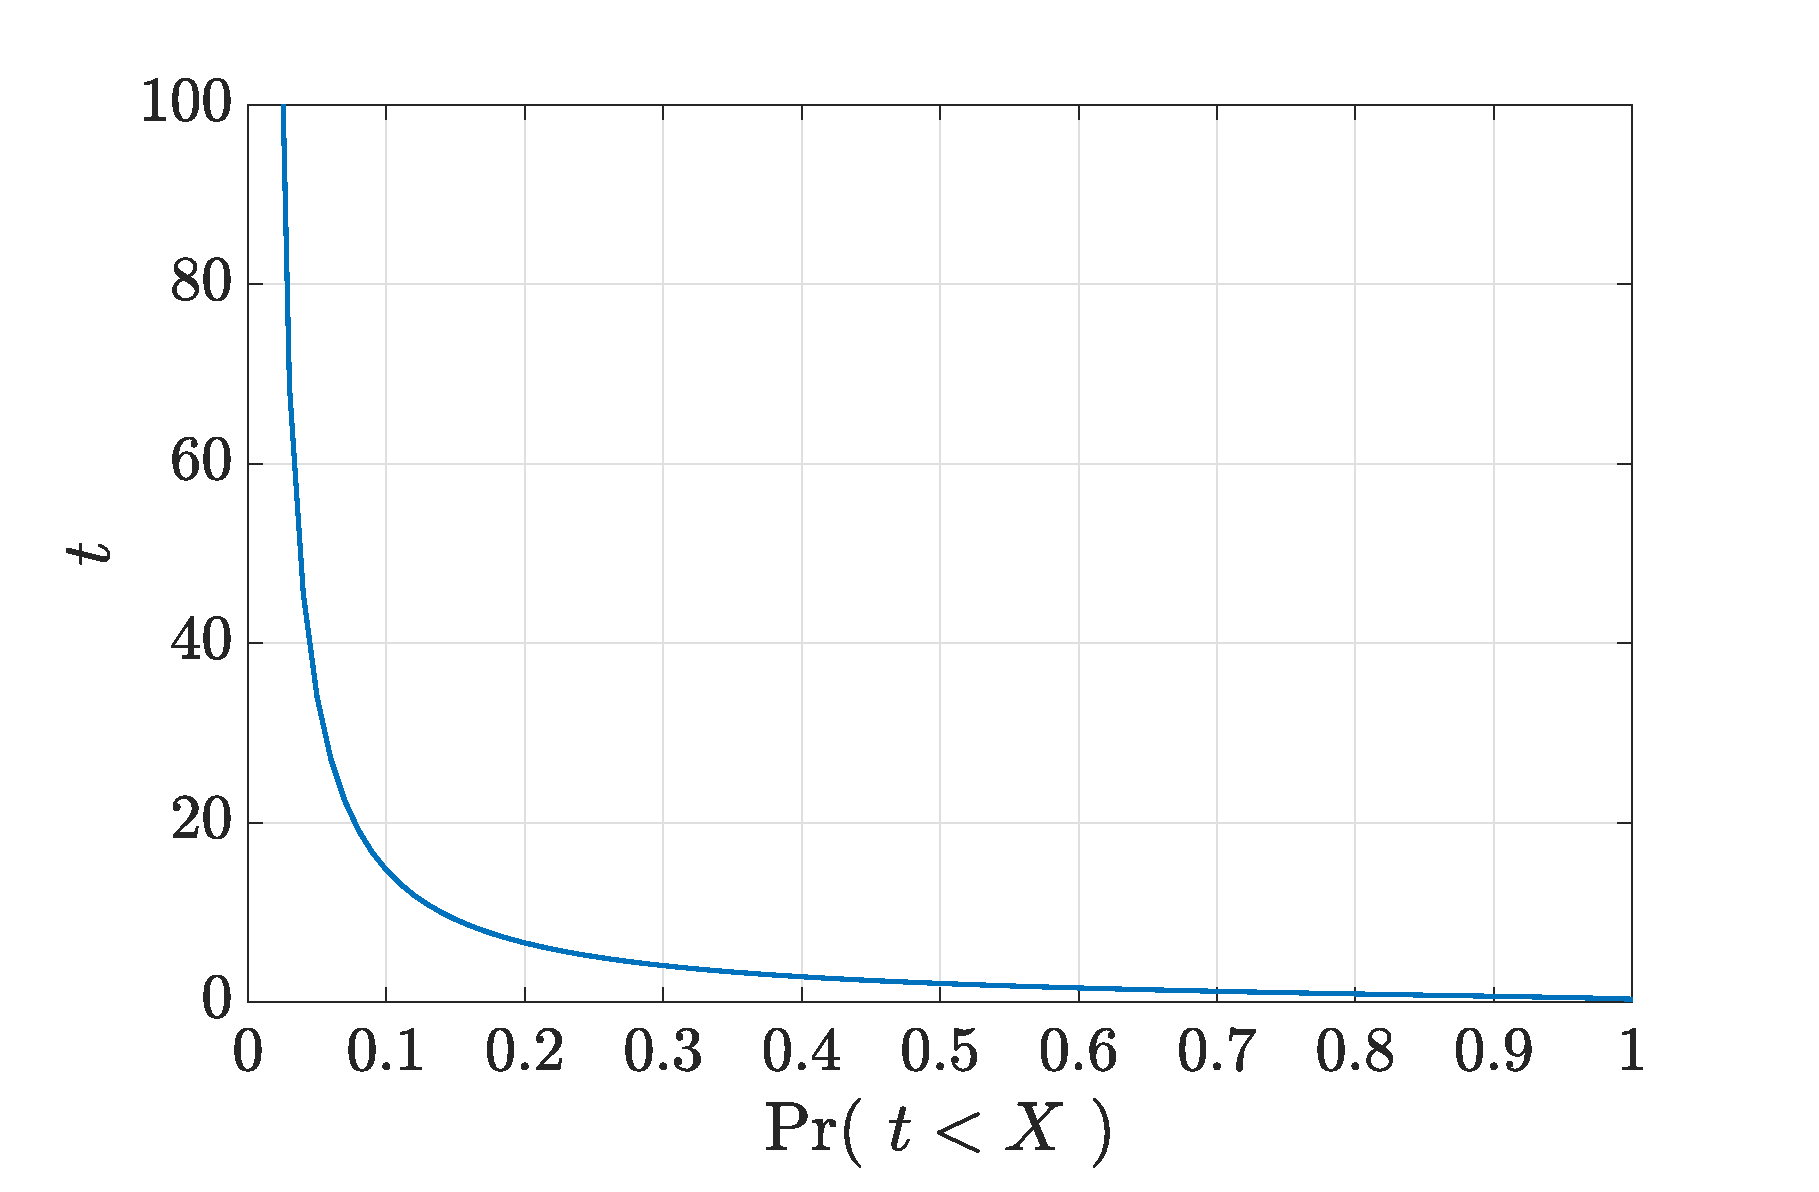
\includegraphics[width = .65\textwidth]{graphs/inverse_chi_square_cdf.eps}}
    \caption{CDF of the inverse chi-square distribution of $\nu = 2$ degrees of freedom.}
    \label{fig:cdf_inverse_chi_square}
\end{figure} 










\subsubsection{LMMSE}
As a recall, the \gls{lmmse} equalizer \textbf{G} needs to satisfy the orthogonality principle. In doing so, we have:
\begin{subequations}
    \begin{align}
         &\EX{(\hat{\textbf{x}}_\text{E} - \textbf{x})\textbf{y}_\text{E}^\text{H}} = \textbf{0} \\
         \Leftrightarrow \; & \EX{(\textbf{G} \textbf{Y}_\text{E}-\textbf{x}) \textbf{y}_\text{E}^\text{H}} = \textbf{0} \\
         \Leftrightarrow \; & \EX{\textbf{G} \textbf{Y}_\text{E} \textbf{y}_\text{E}^\text{H} }  = \EX{\textbf{x} \textbf{y}_\text{E}^\text{H}} \\
         \Leftrightarrow \; & \textbf{G}  = \EX{\textbf{x} \textbf{y}_\text{E}^\text{H}} \left(\EX{\textbf{Y}_\text{E} \textbf{y}_\text{E}^\text{H}}\right)^{-1} \\
         \begin{split}
             \Leftrightarrow \; & \textbf{G}  = \EX{\textbf{x}  \left(   \sqrt{\alpha} \Gamma_{\text{E}} \textbf{x} + \sqrt{1-\alpha} \HE \w + \ve \right)^H }  \\
             & \hspace{.35in} \left(\EX{\left(   \sqrt{\alpha} \Gamma_{\text{E}} \textbf{x} + \sqrt{1-\alpha} \HE \w + \ve \right)\left(   \sqrt{\alpha} \Gamma_{\text{E}} \textbf{x} + \sqrt{1-\alpha} \HE \w + \ve \right)^H}\right)^{-1}
         \end{split}\\
         \begin{split}
            \Leftrightarrow \; & \textbf{G}  = \left(\sqrt{\alpha} \EX{\textbf{xx}^H \Gamma_{\text{E}}^H} + \sqrt{1-\alpha}  \EX{\textbf{x}\w^H \HE^H}  + \EX{x \ve^H}\right) \\
            &\hspace{.35in} \left( \EX{\alpha \Gamma_\text{E} \Gamma_\text{E}^H \textbf{xx}^H + (1-\alpha) \HE \w\w^H\HE^H + \ve\ve^H}\right)^{-1}
         \end{split} \\
         \Leftrightarrow \; & \textbf{G}  = \sqrt{\alpha} \sigma^2_{\text{X}} \Gamma_{\text{E}}^H \left( \alpha \sigma^2_{\text{X}} \Gamma_{\text{E}}\Gamma_{\text{E}}^H  + (1-\alpha) \module{\HE}^2 \sigma^2_{\text{AN}} + \sigma^2_{\text{VE}} \textbf{I}_N\right)^{-1}
    \end{align}
    \label{eq:appA_lmmse}    
\end{subequations}


\newpage
% ANNEXE B : Optimal amout of AN to inject
%\setcounter{figure}{0}
%\setcounter{table}{0}
%\setcounter{section}{0}
%\setcounter{equation}{0}
%\numberwithin{equation}{section}
\renewcommand{\theparagraph}{B}

\section{Optimal amount of AN to inject derivation}\label{appB:alpha}
As a recall, the \gls{sinr} at Bob and Eve are respectively given by:
\begin{equation}
    \begin{split}
        \EX{\gamma_{B,n}} &= \frac{\alpha \;(U+1)}{U \; \sigma_{\text{V,B}}^2} \\
        \EX{\gamma_{E,n}} &= \frac{\alpha}{U(\sigma^2_{\text{V,E}}+(1-\alpha)\sigma^2_{\text{AN}})} 
    \end{split}
\end{equation}
The \gls{sr} becomes:
\begin{subequations}
\begin{align}
    C_s &= \log_2\left(1+ \frac{\alpha (U+1)}{U  \sigma_{\text{V,B}}^2}\right) - \log_2\left(1 + \frac{\alpha}{U(\sigma^2_{\text{V,E}}+(1-\alpha)\sigma^2_{\text{AN}})} \right)\\
    \Leftrightarrow C_s &= \log_2\left( \frac{\alpha (U+1) + U  \sigma_{\text{V,B}}^2}{U  \sigma_{\text{V,B}}^2} \right) - \log_2\left(  \frac{\alpha + U\sigma^2_{\text{V,E}}+(1-\alpha)U\sigma^2_{\text{AN}}}{U\sigma^2_{\text{V,E}}+(1-\alpha)U\sigma^2_{\text{AN}}}  \right)\\
    \Leftrightarrow C_s &= \log_2\left(  \frac{-\alpha^2(U+1)U\sigma^2_{\text{AN}} + \alpha\left[ U(U+1)(\sigma^2_{\text{V,E}}+\sigma^2_{\text{AN}}) - U^2\sigma^2_{\text{V,B}}\sigma^2_{\text{AN}}\right]  + U(\sigma^2_{\text{V,B}}+\sigma^2_{\text{V,E}}+\sigma^2_{\text{AN}})}{\alpha U \sigma^2_{\text{V,B}}(1-U\sigma^2_{\text{AN}}) + U(\sigma^2_{\text{V,B}}+\sigma^2_{\text{V,E}}+\sigma^2_{\text{AN}}) }   \right)
\end{align}
\end{subequations}
If we introduce $T_1=(U+1)U\sigma^2_{\text{AN}}$, $T_2=U(U+1)(\sigma^2_{\text{V,E}}+\sigma^2_{\text{AN}}) - U^2\sigma^2_{\text{V,B}}\sigma^2_{\text{AN}}$, $T_3=U(\sigma^2_{\text{V,B}}+\sigma^2_{\text{V,E}}+\sigma^2_{\text{AN}})$, and $T_4=U \sigma^2_{\text{V,B}}(1-U\sigma^2_{\text{AN}})$, we come back to (\ref{eq:SR_anal2}).

\newpage
% ANNEXE C : Momentum derivation for complex-valued random normal variable 
%\setcounter{figure}{0}
%\setcounter{table}{0}
%\setcounter{section}{0}
%\setcounter{equation}{0}
%\numberwithin{equation}{section}
\renewcommand{\theparagraph}{C}

\section{Momentum computation of complex-valued random normal variables}
\label{appC}
\subsection{Real-valued random normal variable}
For real-valued random variable, the moment-generating function is an alternative specification of its probability distribution. In particular, it allows to compute the moments of the probability distribution as:
\begin{equation}
m_n = \EX{X^n} = M_X^{(n)}(0) = \left. \frac{d^n M_X}{dt^n}\right|_{t=0}
\end{equation}
For a real normal random variable $\mathcal{N}(\mu,\sigma^2) $, the moment-generating function is given by:
\begin{equation}
M_X = e^{t \mu + \frac{1}{2} \sigma^2 t^2 }
\end{equation}
From that, we have:
\begin{equation}
\begin{split}
&\EX{|X|^2} = \sigma^2 + \mu^2\\
&\EX{|X|^4} = 3(\sigma^2)^2 + 6 \sigma^2 \mu^2 + \mu^4
\end{split}
\label{eq:moments_x}
\end{equation}

\subsection{Complex-valued random normal variable}
A complex normal random variable is defined as $Z = X + iY$ where $X \sim \mathcal{N}(\mu_x,\sigma^2_x)$ and $Y \sim \mathcal{N}(\mu_y,\sigma^2_y)$. We also have:
\begin{equation}
\begin{split}
&|Z|^2 = X^2 + Y^2\\
&|Z|^4 = X^4  + 2 X^2 Y^2 + Y^4
\end{split}
\label{eq:deriv_z}
\end{equation}
Since $X$ and $Y$ are independent and taking into account eq.\ref{eq:moments_x}, the moments of $Z$ are easy to compute:
\begin{equation}
\begin{split}
&\EX{|Z|^2} = \sigma_x^2 + \mu_x^2 + \sigma_y^2 + \mu_y^2\\
&\EX{|Z|^4} = 3(\sigma_x^2)^2 + 6 \sigma_x^2 \mu_x^2 + \mu_x^4 + 2\left[ ( \sigma_x^2 + \mu_x^2 )(\sigma_y^2 + \mu_y^2)\right] + 3(\sigma_y^2)^2 + 6 \sigma_y^2 \mu_y^2 + \mu_y^4
\end{split}
\label{eq:moments_z}
\end{equation}






\end{appendices}

\addtocontents{toc}{\vspace{2em}}  % Add a gap in the Contents, for aesthetics

\end{document}










